
\Chapter{\label{CH:challenges}Challenges in data reduction}{Etalon cavity map}

In previous chapters, we have focused on TuMag, its properties, and the correction of its data. However, there are other tunable spectropolarimeters, each with its own specific characteristics, advantages, and challenges. In this chapter, we shift our focus away from TuMag and turn our attention to etalon-based magnetographs in general, with special interest on those with their etalon in a telecentric configuration.

Our interest in studying these kind of instrumentation lies in their extended use in the field of solar physics. Their spectroscopic and tunability properties make them especially suitable for selecting a narrow spectral band of incoming light. They also offer a two-dimensional view of the solar scene, hence allowing for the implementation of powerful and widespread image post-processing reconstruction techniques, such as phase diversity \citep{PD_etalon} and multi-object multi-frame blind deconvolution (MOMFBD; \citealt{mombfd}), which are difficult to implement in slit-based spectrographs (\citealt{image_spectro}, \citealt{image_spectro_2}). Many state-of-the-art instruments use FPIs as narrowband tunable filters. Among others, these instruments include the spaceborne Polarimetric and Helioseismic Imager \citep[][]{PHI} aboard the Solar Orbiter mission \citep[][]{SO} (SO/PHI); the Imaging Magnetograph Experiment (IMaX) instrument \citep[][]{IMaX}, which flew on the first two flights of the balloon-born SUNRISE observatory (\citealt{SunriseI}, \citealt{SunriseII}); and the Tunable Magnetograph (TuMag) instrument for its third edition. These instruments are based on solid LiNbO$_3$ etalons. Regarding ground-based instruments, some examples include the Crisp Imaging Spectro-Polarimeter (CRISP) at the Swedish 1-m Solar telescope \citep[][]{crisp} at the Observatorio del Roque de los Muchachos in La Palma, Canary Islands; the GREGOR Fabry-Perot Interferometer (GFPI; \citealt{GFPI}, \citealt{GREGOR}) at the Observatorio del Teide in Tenerife, Canary Islands; the Visible Tunable Filter \citep[VTF;][]{VTF} developed for the \textit{Daniel K. Inouye} Solar Telescope \citep[DKIST;][]{DKIST} of the Haleakal\=a Observatory in Hawaii; and the future Tunable Imaging Spectropolarimeter (TIS) of the European Solar Telescope \citep{EST}, all of which are based on air-gapped etalons. 

Currently, there is an ongoing debate within the scientific community regarding the optimal optical configuration for the etalon in spectropolarimeters, whether it should be collimated or telecentric. Since the seminal work of \citealt{beckers} where they carried an analysis of the optical performance of FPIs, the debate has garnered significant interest, as evidenced by the numerous studies addressing the properties of each configuration. Notable contributions include the four works by Bailén et al. (\citealt{franI}, \citealt{franII}, \citealt{franIII}, \citealt{franIV}), an extensive analysis on topics such as the impact of defects, applications for instrumentation, and the analytical formulation of the etalon's transmission profiles. Other examples include the studies of \cite{ghosts-etalon}, a detailed assessment of the comparison in optical performance between configurations, as well as the works of \citealt{kentischer1998tesos} and \citealt{cavallini2006ibis}, which discuss the properties of the etalons in the Telecentric Etalon Solar Spectropolarimeter (TESOS) and the Interferometric BIdimensional Spectrometer (IBIS), respectively. Additionally, the review of \citealt{ghosts-etalon} provides a broad and comprehensive overview of this topic. The reality is that it is challenging to provide a definitive answer to this question, as each configuration has its own advantages and disadvantages.

The primary argument against collimated mounts is the amplification of wavefront errors resulting from the large footprint of the light rays on the etalon plates, which includes both large and small scale defects \citep{fran_review}. This amplification deteriorates the optical quality of these setups and has promoted the use of telecentric setups, where the footprints of the light rays are much smaller and the optical performance is less affected by large scale defects.

Despite the improvement in optical performance, the telecentric configuration is no exempt of challenges. In this configuration each light ray trasverses the etalon through different regions, thus being affected differently at each point from the various small scale defects present in the etalon. This defects, compose the so-called, cavity-map and its correction can be one of the main challenges of employing these setups.

This chapter aims to provide a description of telecentric configurations for etalons within the context of solar spectropolarimeters. We will begin by exploring the analytical formulation of the transmission profiles and spatial PSF of FPI's in both collimated and telecentric configurations. Following this, we will delve into the effects of the cavity error in solar observations, through a simulation of an observation of a Sunspot. Then, we will present a strategy to derive the cavity map from flat field observations in an attempt to improve the data correction. 

\section{One device, two configurations.}

We established in section \ref{sec: intro-imaging} that the observed intensity distribution at the coordinates $\xi$, $\eta$ of the focal plane of any etalon-based instrument tuned to a wavelength $\lambda_s$ obeys the following expression \citep{franI}: 

\begin{equation}
    I\left(\xi, \eta ; \lambda_{s}\right)=g(\xi, \eta)\int_{0}^{\infty} T(\lambda) \iint  O\left(\xi_0, \eta_0 ; \lambda\right)  \mathcal{S}\left(\xi_0, \eta_0; \xi , \eta; \lambda-\lambda_{s}\right)  \mathrm{d} \xi_{0} \mathrm{~d} \eta_{0}\mathrm{d} \lambda ,
    \label{eq_etalon_theory: General_Intensity}
\end{equation}
where $T(\lambda)$ accounts for the transmission of the order-sorting pre-filter, $O\left(\xi_0, \eta_0 ; \lambda\right)$ represents the brightness distribution of the observed object at the point $\left(\xi_0, \eta_0\right)$ and wavelengths $\lambda$, $S\left(\xi_0, \eta_0; \xi , \eta; \lambda-\lambda_{s}\right)$ accounts for the imaging response of the instrument when tuned at the wavelength $\lambda_{s}$, and $g(\xi, \eta)$ represents a spatial gain factor that accounts for wavelength independent pixel-to-pixel intensity fluctuations ocurring in the focal plane due to differences in the detectors' sensitivity. 

The imaging response of the instrument coincides with the PSF of the instrument when the optical response is invariant against translations. In such a case, we can express the imaging response as: $S =\mathcal{S}\left(\xi - \xi_0 , \eta - \eta_0; \lambda-\lambda_{s}\right)$, and also substitute the last two integrals by the convolution operator.  However, this is not strictly true in etalon-based instruments, where the response varies pixel to pixel either because of etalon irregularities or because of variations in the illumination across its clear aperture.

Deriving S requires determining the electric field of the polychromatic wave in the image plane. This field can be calculated by Fourier transforming the electric field $E^{(t)}$ across the pupil, such that the electric field at any point $(\xi, \eta)$ of the image plane follows the expression \citep{franI}:

\begin{equation}
  E  ^{(t)}(\xi, \eta) = \frac{1}{\pi R_{pup} ^2} \int \int _ {pup} E^{(t)}(x, y)e ^{-ik( \xi x / f + \eta y / f)}dx dy,
  \label{eq_etalon_theory: electric_image_plane}
\end{equation}
where $(x, y)$ are the coordinates over the pupil, $f$ stands for the focal length, and $R_{pup}$ is the radius of the pupil.  It can also be shown that the vector electric fields transmitted by the etalon can be expressed as:

\begin{equation}
  E ^{(t)}(\xi, \eta) = \frac{\sqrt{\tau}}{1 - R}\frac{e ^{i\delta / 2} - R e ^{ -i\delta / 2}}{1 + F \sin ^2 (\delta / 2)}E ^{(i)},
  \label{eq_etalon_theory: electric_transmitted}
\end{equation}
where $\tau$ is the transmission factor for normal incidence, $R$ stands for the reflectivity of the etalon mirrors, $F$ is a factor defined as $F \equiv 4R (1 - R )^{-2}$, $E^{(i)}$ are the incident electric fields, and $\delta$ stands for the phase differences between the transmitted and incident rays. 

The transmission profile of the etalon $S$ is defined as the average ratio between the transmitted and incident intensities, calculated from the complex conjugate of the corresponding electric fields. The dependence of $\delta$ with the coordinates $(\xi, \eta)$ varies depending on the illumination setup of the etalon, whether collimated or telecentric. Consequently, each configuration has a unique response and is differently affected by inhomogeneities (defects) in the etalon's properties.

\subsection{\label{susec_etalon_theory: collimated}Collimated configuration}

\begin{figure}
  \centering
  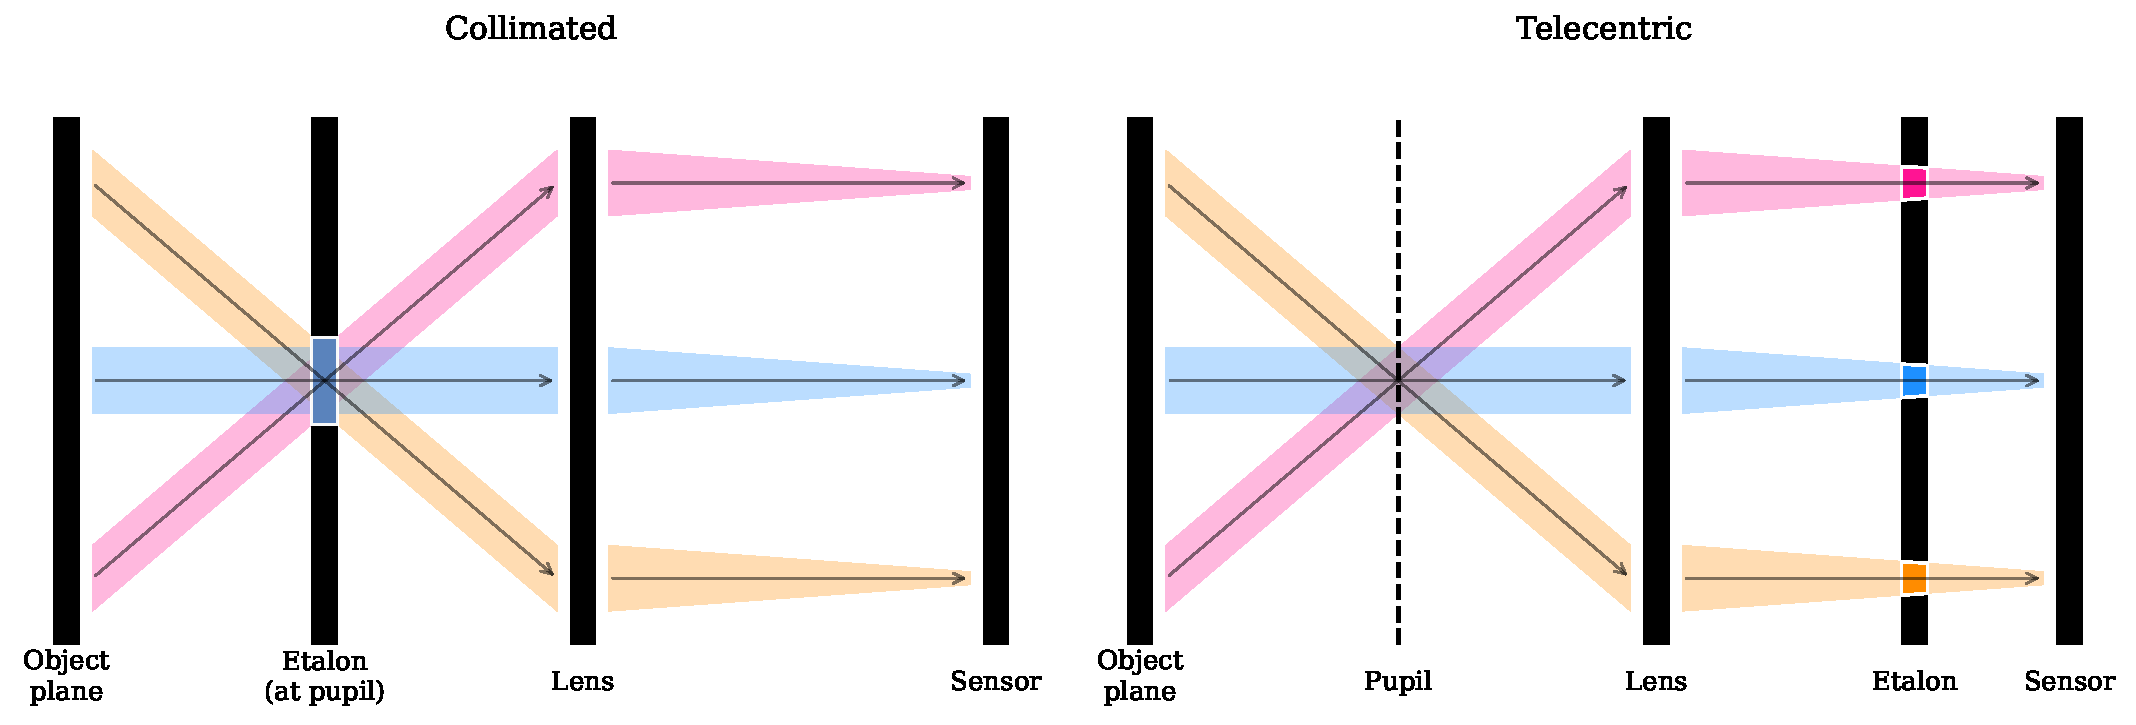
\includegraphics[width = \textwidth]{figures/EtalonChallenges/EtalonConfigurations.pdf}
  \caption[Etalon's configuration schematic.]{Schematic representation of the two optical setups of an FPI, collimated (left) and telecentric (right). The different colors represent distinct light rays originating from various points on the object plane. The white boxes in the etalon highlight the sections that are traversed by the light rays.
  } \label{fig_etalon_theory: Etalon configurations}
\end{figure}

Collimated mounts are characterized for having the etalon located at the pupil plane placed in collimated space and therefore receive a collimated beam with different incidence angles for each point of the observed object. As illustrated in the schematic on the left side of fig.~{\ref{fig_etalon_theory: Etalon configurations}}, light from any point on the object will illuminate the same area of the etalon. Consequently, any local defects on the etalon cavities or on the plates' parallelism are averaged all over the clear aperture, thus making the optical quality constant along the FoV. However, the angle of incidence of the light beam varies along the FoV, thus shifting the spectral transmission profile.  

Analytical solutions of equation \eqref{eq_etalon_theory: electric_image_plane} are imposible to obtain if $\delta$ has a dependence on the pupil coordinates, as is the case of collimated etalons with a presence of local defects. In that case, the wavelength-dependent PSF of the etalon has to be evaluated numerically. 

However, in order to study the spectral behavior of the PSF, we can, as a first-order approximation, disregard the spatial PSF and focus solely on the spectral transmission profile $\psi$. Under this assumption, the phase difference between the incident and transmitted rays of an ideal collimated etalon can be expressed as:  

\begin{equation}
  \delta (\xi, \eta, \lambda) = \frac{4\pi}{\lambda}nd\cos (\theta(\xi, \eta)),
  \label{eq_etalon_theory: collimated_delta}
\end{equation}
where $n$ stands for the refractive index of the etalon cavity, $d$ is the distance between the mirrors and $\theta$ is the angle of incidence. In such a case, the spectral transmission profile can be obtained from $E ^{(t)}\ E^{(t)*}$, where the asterisk indicates the complex conjugate, and follows the expression: 

\begin{equation}
  \psi\left(\xi, \eta, \lambda \right) = \frac{\tau}{1 + F \sin ^2 (\delta(\xi, \eta, \lambda) / 2)}.
  \label{eq_eta_theory : Collimated_profile}
\end{equation}

The spectral behaviour of the transmission profile, such as the spectral position of the resonance peaks and the distance between them (the free spectral range), is encoded in the parameter $\delta$, which is a function of the refractive index of the etalon cavity, the distance between mirrors, and the angle of the incident beam. The reflectivity $R$ of the mirrors determines the width of the resonance peaks through the parameter $F$, $F \equiv 4R (1 - R )^{-2}$.

Local defects in the collimated configuration are averaged out, which means that $d$ and $n$ respectively represent the mean values of the thickness and refractive index across the clear aperture of the FPI, and thus remain constant for every pixel. Yet, they produce a broadening of the transmission profile and worsen the optical quality of the instrument. However, the spatial dependence of $\psi$ naturally arises from $\theta$, which varies from pixel to pixel. 

Assessing the spatial PSF of the FPI is more challenging, as it can only be determined analytically for monochromatic light and in the absence of defects. We will not delve into the equations for this specific scenario as it lies beyond the scope of this thesis. However, interested readers are referred to the work of \cite{fran_review}, where this topic is extensively discussed.

\subsection{\label{susec_etalon_theory: Tele-perfe}Telecentric configuration}

In the telecentric configuration, the etalon is placed very close to an intermediate focal plane, while the pupil is focused at infinity. As shown in the sketch on the right side of fig.~{\ref{fig_etalon_theory: Etalon configurations}}, in this setup, the etalon is illuminated by cones of rays that are parallel to each other, thus passing through different sections of the interferometer. Local inhomogeneities (defects or cavities) on the etalon produce differences in the transmission profile across the FoV, which are directly mapped into the image plane. This means that the optical response and the transmission profile shift locally over the image plane. 

In telecentric configurations, $\delta$ always depends on the coordinates of the pupil, even in the absence of defects, since each point in the etalon sees a cone of rays coming from different parts of the pupil. Thus, as stated before, solutions to equation \eqref{eq_etalon_theory: electric_image_plane} are to be found numerically. Nonetheless, if we neglect the spatial PSF once again, we can derive an analytical expression for an ideal telecentric etalon, where all light cones impact perpendicularly.

It is possible to recast eq. \eqref{eq_etalon_theory: electric_image_plane} in terms of the radial coordinates of the pupil and analytically solve the equations. The resulting spectral transmission profile of an ideal telecentric etalon  is given by \citep{franIV}:
\begin{equation}
\Psi \left(\xi, \eta, \lambda \right) =  \mathfrak{Re}\left[E(a\left(\xi, \eta, \lambda \right), b\left(\xi, \eta, \lambda \right)) \right] ^2 + \mathfrak{Im}\left[E(a\left(\xi, \eta, \lambda \right), b\left(\xi, \eta, \lambda \right)) \right] ^2 ,
\label{eq_etalon_theory: Tel_first}
\end{equation}
with $E(a\left(\xi, \eta, \lambda \right), b\left(\xi, \eta \right))$ being:
\begin{multline}
E(a\left(\xi, \eta, \lambda \right), b\left(\xi, \eta \right)) = 2\sqrt{\tau}\Biggl\{ \frac{1}{\alpha_1}\left[\arctan(\gamma _ 1) - \arctan(\gamma_2)\right] + \\
\mathrm{i} \frac{1+R}{1-R} \frac{1}{\alpha_2}\left[\ln \left(\frac{(1 + \gamma _ 3) ^2 + \gamma _ 4 ^2}{(1 - \gamma _ 3) ^2 + \gamma _ 4 ^2} \right) - \ln \left(\frac{(1 + \gamma_ 3) ^2 + \gamma _ 5 ^ 2}{(1 - \gamma _ 3) ^2 + \gamma _ 5 ^2} \right)\right]\Biggr\},  
\end{multline}
where, the auxiliary functions are defined as:
\begin{equation}
\begin{split}
a\left(\xi, \eta, \lambda \right) &\equiv \frac{2 \pi}{\lambda}n\left(\xi, \eta\right)d\left(\xi, \eta\right) \ , \\
b\left(\xi, \eta\right) &\equiv \frac{1}{8n\left(\xi, \eta\right)^2(f\#) ^2}\ ,  \\
\alpha _ 1 &\equiv 2ab\sqrt{F}\ ,  \\
\alpha _ 2 &\equiv 2\alpha_ 1\sqrt{F + 1}\ ,  \\
\gamma _ 1 &\equiv \sqrt{F} \sin a\ ,  \\
\gamma _ 2 &\equiv \sqrt{F} \sin (a[1 - b])\ ,  \\
\gamma _ 3 &\equiv \sqrt{\frac{F}{F + 1}} \ ,  \\
\gamma _ 4 &\equiv \frac{\tan \left( a/2 [1 - b] \right)}{\sqrt{F + 1}}\ ,  \\
\gamma _ 5 &\equiv \frac{\tan (a/2)}{\sqrt{F + 1}}\ .
\end{split}
\end{equation}

The parameter $a$ has the same role as $\delta$ for the collimated case. However, the dependence on the image plane coordinates in this case is caused by potential variations in n and/or d, as each light beam traverses different sections of the etalon. These variations constitute the so-called "cavity map" of a telecentric etalon and must always be taken into account during data reduction processes.

The parameter $b$ accounts for the contribution of the focal ratio, $f\#$, and has an impact on the spectral resolution, among other effects \citep{beckers}. Thus, the resolution is affected by both $F$ and $f\#$, through the parameters $a$ and $b$.

\subsubsection{\label{etalon_theory: Tele-imperfe}Telecentric imperfect configuration}
The equations shown in Sect.~\ref{susec_etalon_theory: Tele-perfe} are valid whenever the incident cone of rays is perpendicular to the etalon mirrors. We refer to this situation hereinafter as "perfect telecentrism". However, real instruments are likely to present deviations from such an ideal case. These deviations can be caused by an intentional tilt of the etalon to suppress ghost images on the detector \citep{ghosts-etalon}, by an accidental off-axis incidence caused by deviations from the ideal paraxial propagation of rays within the instrument, or simply because of misalignment of the optical components. In the three cases, the incident cone of rays is no longer perpendicular to the etalon, and hence, we consider these scenarios as if they were imperfections in the telecentrism degree. One important consequence of the loss of telecentrism is an asymmetrization of the transmission profile that must be accounted for when modeling the instrument response.

The transmission profile in this case is influenced by the angle of incidence of the chief ray at each point of the clear aperture of the etalon, in addition to the parameters mentioned in the previous sections. Unfortunately, the equations for the transmission profile in these configurations are much more complicated than in the ideal case, and can no longer be analytically solved. We must revisit equation \eqref{eq_etalon_theory: electric_image_plane} and solve the integrals numerically.

\begin{figure}
    \centering
    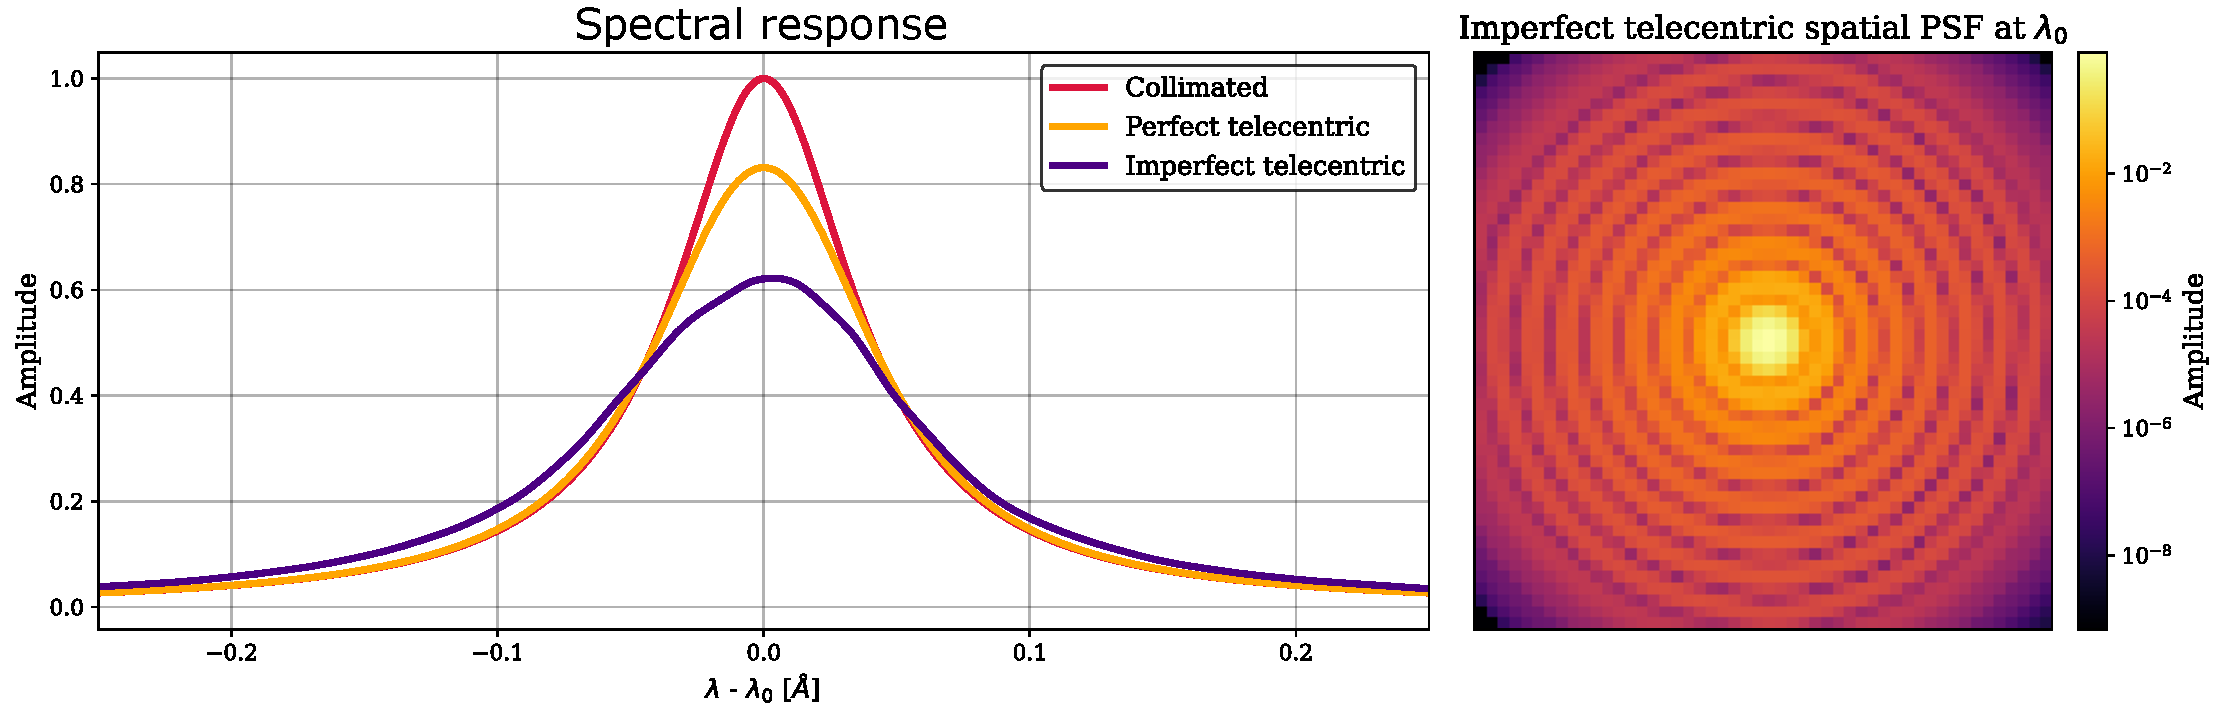
\includegraphics[width = \textwidth]{figures/EtalonChallenges/etalon_setups_profiles.pdf}
    \caption[Etalon's spectral and spatial PSFs.]{\textit{Left}: central peak of the etalon's spectral transmission profile for the three different configurations. \textit{Right}: Spatial PSF of the imperfect telecentric etalon at $\lambda _ 0$. The parameters of the etalon are $R = 0.92$, $n = 2.29$, $d = 251 \, \mu \mathrm{m}$, $f\#=56$, $\theta = 0 ^{\circ}$ (collimated and perfect telecentric), and $\Theta = 0.3\,^{\circ}$ (imperfect telecentric).}
    \label{fig_etalon_theory:Profiles-configs}
\end{figure}

Figure \ref{fig_etalon_theory:Profiles-configs} shows on the left the transmission profile corresponding to the three different scenarios: collimated illumination of the etalon, perfect telecentrism, and imperfect telecentrism. The etalon parameters have been selected to coincide with those of SO/PHI's etalon. In both the collimated and perfect telecentric configurations, a normal incidence  ($\theta = 0$) scenario is shown, whereas in the imperfect telecentric case, we assumed an angle of incidence of the chief ray, $\Theta$, of $0.3^{\circ}$. The parameter $a$ has been adjusted slightly in order to tune the transmission profile at $\lambda _ 0$. 

Regarding the properties of each profile, note that the telecentric configurations achieve lower peak transmissions than the collimated case. In addition, the telecentric profiles are wider due to the different incidence angles across the illuminating cone of rays. Such a broadening increases with decreasing f-ratios. Lastly, non-normal incidence of the chief ray in the telecentric configuration further widens and shifts ($\sim 4$~m\r{A} for $\Theta=0.3^\circ$) the profile, in addition to making it asymmetrical. 

\section{\label{sect: Mancha_obs}Sunspot observation simulation}

The analytical formulations provide us with the necessary tools to investigate the impact of the cavity map on observational data and the consequences of incorrect or incomplete corrections. Our objective is to quantify the spurious effects of the cavity map on scientific products, specifically LOS velocities and magnetic field strength. To achieve this, we will simulate a series of sunspot observations using a telecentric FPI and attempt to correct these observations.

The simulations are carried out introducing cavity errors to the etalon and accounting for gain variations across the cameras' FoV. To accurately reflect the real scenario, the data will require flat-field correction before analysis. Consequently, we will simulate not only the scientific observations but also the flat-field observations. The following sections detail the process for the simulation of both the sunspot observations and the flat-fields.

We have chosen to employ a sunspot for this study since they are one of our main \textit{laboratories} for the study of the magnetic field and dynamics of the solar photosphere. Additionally, they exibit complex and diverse structures that facilitate the identification of etalon effects on observations as a function of solar structure. Sunspots are dark regions of the solar surface where strong magnetic fields gather. The innermost part of the spot, the umbra, with a brightness around the 20$\%$ of its surroundings, hosts very strong magnetic fields oriented almost perpendicular to the solar's surface. Surrounding the umbra in fully developed sunspots is the penumbra, a brighter region characterized by a radial filamentary structure with a nearly horizontal outflow of the plasma known as the Evershed flow \citep{evershed}. 

The physical mechanisms driving the phenomena in these regions are not yet fully understood and have been a topic of discussion for many years, and still are. Processes such as the Evershed flow lack a universally accepted theoretical model, and numerous studies attempt to provide a theoretical basis for the observations, often presenting conflicting interpretations. Some examples of these works are \cite{evershed_magnetic_flux}, or \cite{evershed_magnetic_2}, where they interpret the evershed flow as a hot gas confinded to magnetic flux tubes that rise due to convecion processes. In contrast, alternative models such as the one proposed by \cite{evershed_model_scharmer} and \cite{evershed_model_spruit}, and later updated in \cite{evershed_magnetic_scharmer}, suggest that the observed filaments are field-free gaps where standard convection occurs. According to these models, the convective cells are elongated as the upward flow is redirected by the inclined magnetic field characteristic of the penumbra, resulting in the outward flow.  

Accurate measurements of velocities and magnetic fields are of paramount importance for deciphering these processes, as the weak and small-scale manifestations of these effects may be crucial for their understanding. Examples for this are the works of \citealt{lateral_downflows_2} or \citealt{lateral_downflows}, where they found and study lateral downflows at the edge of penumbral filaments, supporting the model of penumbral convection from filament dynamics. However, these downflows are very challenging to detect, and require very high spatial resolution and accurate velocity measurements. For this reason, we will focus on the study of the spurious effects of the cavity error in the measurements of velocities and magnetic fields, with a special emphasis on penumbral flows. 

The target of our observations will be a Magnetohydrodynamic (MHD) simulation of a sunspot in the photosphere kindly provided by C. Quintero Noda. We will observe it through an FPI similar to the one flying aboard the SO as part of the PHI instrument. This section begins with an overview of the simulated data (Sect.\ref{sect: mancha_sim_data}), followed by a detailed explanation of the observation simulation (Sect.\ref{sect: mancha_obs_sim}). Subsequently, we present and discuss the different flat-fielding strategies in section \ref{sect: mancha_ff_corr}. The section concludes with the discussion of the measurements of the LOS velocities and magnetic field strength in sections \ref{sect: mancha_vlos} and \ref{sect: mancha_blos}, respectively.  


\subsection{\label{sect: mancha_sim_data}Simulated data.}

The target of the observations is a MHD simulation of a sunspot taken from \cite{mancha-seminal}. These simulations, generated using the MuRaM code \citep{MURaM}, were employed to synthesize the Stokes profiles with the SIR code \citep{sir}.  Specifically, we utilize a simulation with dimensions of 1536×128×1536 pixels, with a grid spacing of 32 km in the horizontal direction and 16 km in the vertical.The spectral synthesis was performed with a sampling of 10 m\r{A}/pixel across a range from -1500 to 1500 m\r{A} relative to the Fe I 6173\r{A} line core. For a detailed description of the simulation we refer the reader to \cite{mancha-carlos}.

As explained in previous chapters, tunable spectropolarimeters do not measure the stokes components directly, but rather infer it from a series of independent measurements. In order to replicate this behaviour, we generated four modulations from the MHD simulations employing an ideal modulation matrix. The images are demodulated using an ideal demodulation matrix, obtained by directly inverting the modulation matrix. This ensures that the results are free from any cross-talk contamination.
\subsection{\label{sect: mancha_obs_sim}Observations simulation.}

All the instruments built around the use of an etalon as the wavelength-selector element operate in a very similar way. They scan a spectral line by tuning the etalon (by changing the distance between mirrors and/or by applying a voltage to modify the refractive index) to a desired number of wavelengths along the spectral line. At each spectral position, the solar scene is recorded. The measured intensity is approximately given by Eq.~\eqref{eq_etalon_theory: General_Intensity}, with the etalon's transmission profile centered at the desired wavelength.

We have carried out two sets of simulations, one with a perfect telecentric configuration, where the incidence of the chief ray is normal to the etalon's surface, and one with an angle of incidence of the chief ray of $0.5^\circ$, that is, with a telecentric imperfect configuration. For both sets a simulation of the whole spectral scan is carried out. For these scans, the 6173 \r{A} spectral line is sampled with 45 wavelengths from - 500 m\r{A} to + 500 m\r{A}, relative to the line's core rest position, in steps of 10 m\r{A}. At each spectral position, the solar scene is recorded for each of the four generated modulations.

These measurements are performed following equation \eqref{eq_etalon_theory: General_Intensity} with the omission of the pre-filter. In practice, it is not often possible to fully characterize the pre-filter, and therefore, for these simulations, we assumed it has a rectangular shape centered at the wavelength of the observed spectral line ($\lambda _ {0}$) and a width of $2\Delta \lambda$ such that only one order of the etalon passes through. With this consideration, equation \eqref{eq_eta_corr: intensity} can be written as follows:

\begin{equation}
  I\left(\xi, \eta ; \lambda_{s}\right)=g(\xi, \eta)\int_{\lambda _ 0 - \Delta \lambda}^{\lambda _ 0 - \Delta \lambda} \iint  O\left(\xi_0, \eta_0 ; \lambda\right)  \mathcal{S}\left(\xi_0, \eta_0; \xi , \eta; \lambda-\lambda_{s}\right)  \mathrm{d} \xi_{0} \mathrm{~d} \eta_{0}\mathrm{d} \lambda \ .
  \label{eq_mancha: Intensity}
\end{equation}

In order to replicate the behaviour of real instrumentation we have introduced a gain variation and cavity errors. The former is straightforward to introduce as it is considered independently in Eq.~\eqref{eq_mancha: Intensity} as a pixel-dependent multiplicative factor that affects the whole mesurement, $g$. In contrast, the effects of the cavity map are more convoluted. Pixel-to-pixel variations in etalon defects shift the transmission profile of the FPI and must be accounted for when computing the imaging response. Both the gain and cavity map introduced in the simulations have been selected to resemble the real-case scenario of the SO/PHI instrument. The gain map (Fig. ~\ref{fig_mancha: Inputs} top right panel) utilized in the simulations is derived from a flat field of the SO/PHI-HRT instrument, and the cavity map employed (Fig. ~\ref{fig_mancha: Inputs} top central panel) is sourced from the cavity map of PHI's etalon.

We see from equation \eqref{eq_mancha: Intensity} that the FPI's imaging response, $\mathcal{S}$, has to be computed for every wavelength and every pixel, since the cavity error varies along the FoV. This is achieved by solving the integrals in equation \eqref{eq_etalon_theory: electric_image_plane} via numerical methods,since we will account for the PSF in these simulations. Consequently, the computational burden is significant, as the integrals must be evaluated $N_{pixel} ^2 N_{\lambda} N_{mods} N_{etalons} N_{cavities} > 2\times10 ^8$ times\footnote[2]{$N_{pixels} = 561$, $N_{\lambda} = 45$, $N_{mods} = 4$, $N_{etalons} = 2$, $N_{cavities} = 2$} for both sunspot and flat field observations. This extensive computation results in excessively long simulation times. To address this issue, a neural network was developed to reduce the computational time from 12 s to 5 ms, more than a factor $2\times10 ^3$ faster, before applying paralellization techniques which will increase the factor to values higher than $10^{5}$.  

The neural network is an implicit neural representation with periodic activation functions (SIREN; \citealt{siren}) trained by A. Asensio Ramos with solutions to the integrals for a fixed set of etalon parameters, namely, spectral ranges, angles of incidence and reflectivity. The solutions provided by the network are accurate up to a 1\% for the etalon parameters within the training set. 

\subsubsection{Flat-field observation simulation.}

As with real observations, sunspot observations have to be flat-fielded before scientific analysis in order to correct for the effects of the gain and, in principle, of the cavity error. In order to reproduce this, we are required to simulate the flat-field observations as well. In real operations, flat-fields are but another set of observations, sharing similar properties in terms of spectral sampling and modulation schemes but target a uniform, structure-free region. To create these observations, we applied the same observation procedure used for the sunspot data to a simulated ideal flat region. This target was generated by averaging the spectral profile of a quiet Sun region from the simulation and replicating it across the entire FoV, producing a completely homogeneous flat-field where every pixel reproduces the quiet Sun's average spectral profile.

Since the main goal of these tests is to assess the impact of incomplete corrections of the cavity map, we conducted all simulations under two scenarios: one incorporating the cavity error and another assuming a defect-free etalon. The latter will serve us as a reference of an observation devoid from any etalon-induced defect, but with identical spectral and spatial degradations. 

\begin{figure}[t]
    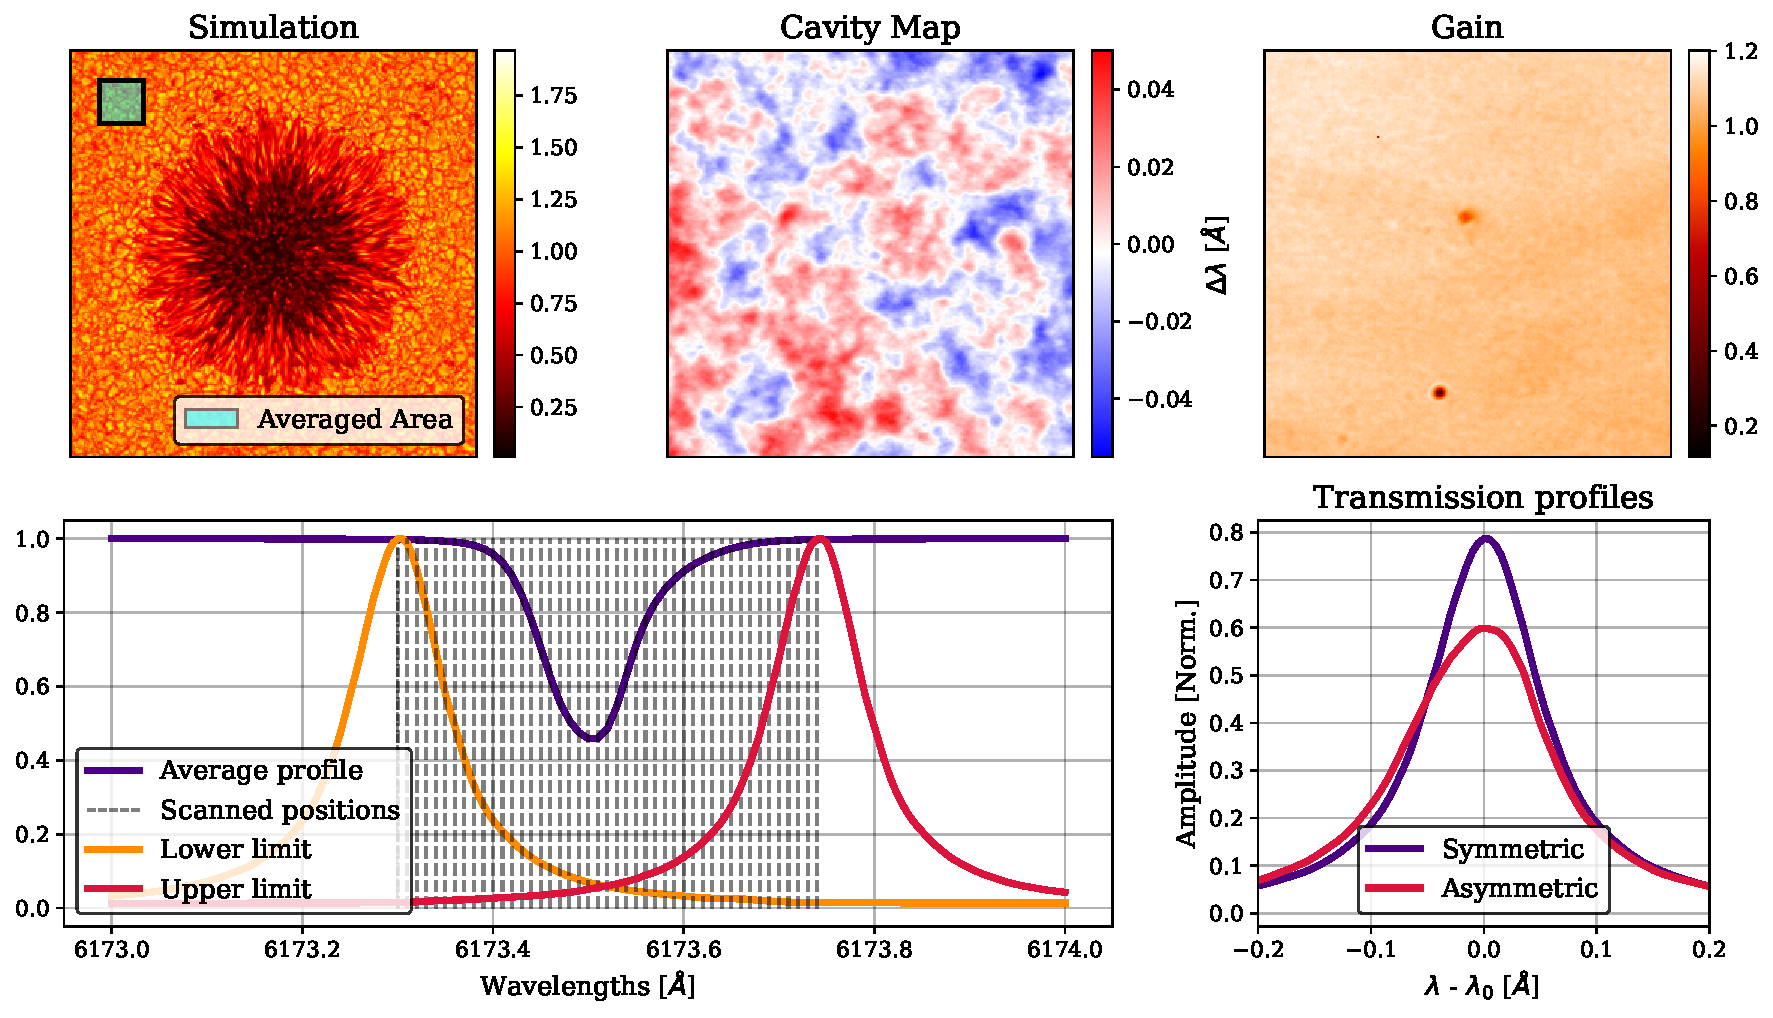
\includegraphics[width=\textwidth]{figures/Mancha/Inputs_mancha.pdf}
    \caption[Sunspot simulation inputs.]{
      Inputs for the simulation of the sunspot observation. The top row shows, from left to right, the continuum of the MHD simulation, the cavity map expressed as the corresponding shift in \r{A} and the gain map. The bottom row shows, again from left to right, a representation of the quiet-sun average profile with all the scanned wavelengths, and the transmission profile of the two different FPI configurations, the symmetric (perfect telecentric) and asymmetric (imperfect telecentric). The parameters employed for the etalon are: $R=0.892$, $n = 2.3268$, $d = 281$ $\mu m$, $f = 60$, $\Theta = 0^{\circ}$ (symmetric), $\Theta = 0.5^{\circ}$ (asymmetric).
      \label{fig_mancha: Inputs}}
\end{figure}

\subsection{\label{sect: mancha_ff_corr}Flat-field correction.}

In principle, any flat-field correction should be straightforward as long as the flat-field information is not altered during the science observation. In the first place, the spectral line information has to be removed from the flat-field observations. To do this, a region of the flat is chosen and each of the wavelengths is normalized to the average of the flat observation in that region. This removes the spectral line contribution to the flat. Then, the observations for all tuned wavelengths are divided by the corresponding normalized flat field. However, in telecentric setups, this process is challenging because flat-field observations are influenced differently from the observations by cavity errors because the illumination (telecentric) on the etalon is different. This is clearly seen in equation Eq-~\eqref{eq_mancha: Intensity} where the response depends on the object O. Hence, the flatfielding can introduce additional artifacts into the measurements rather than (or in addition to) correcting them.

\begin{figure}
  \begin{minipage}[c]{0.7\textwidth}
    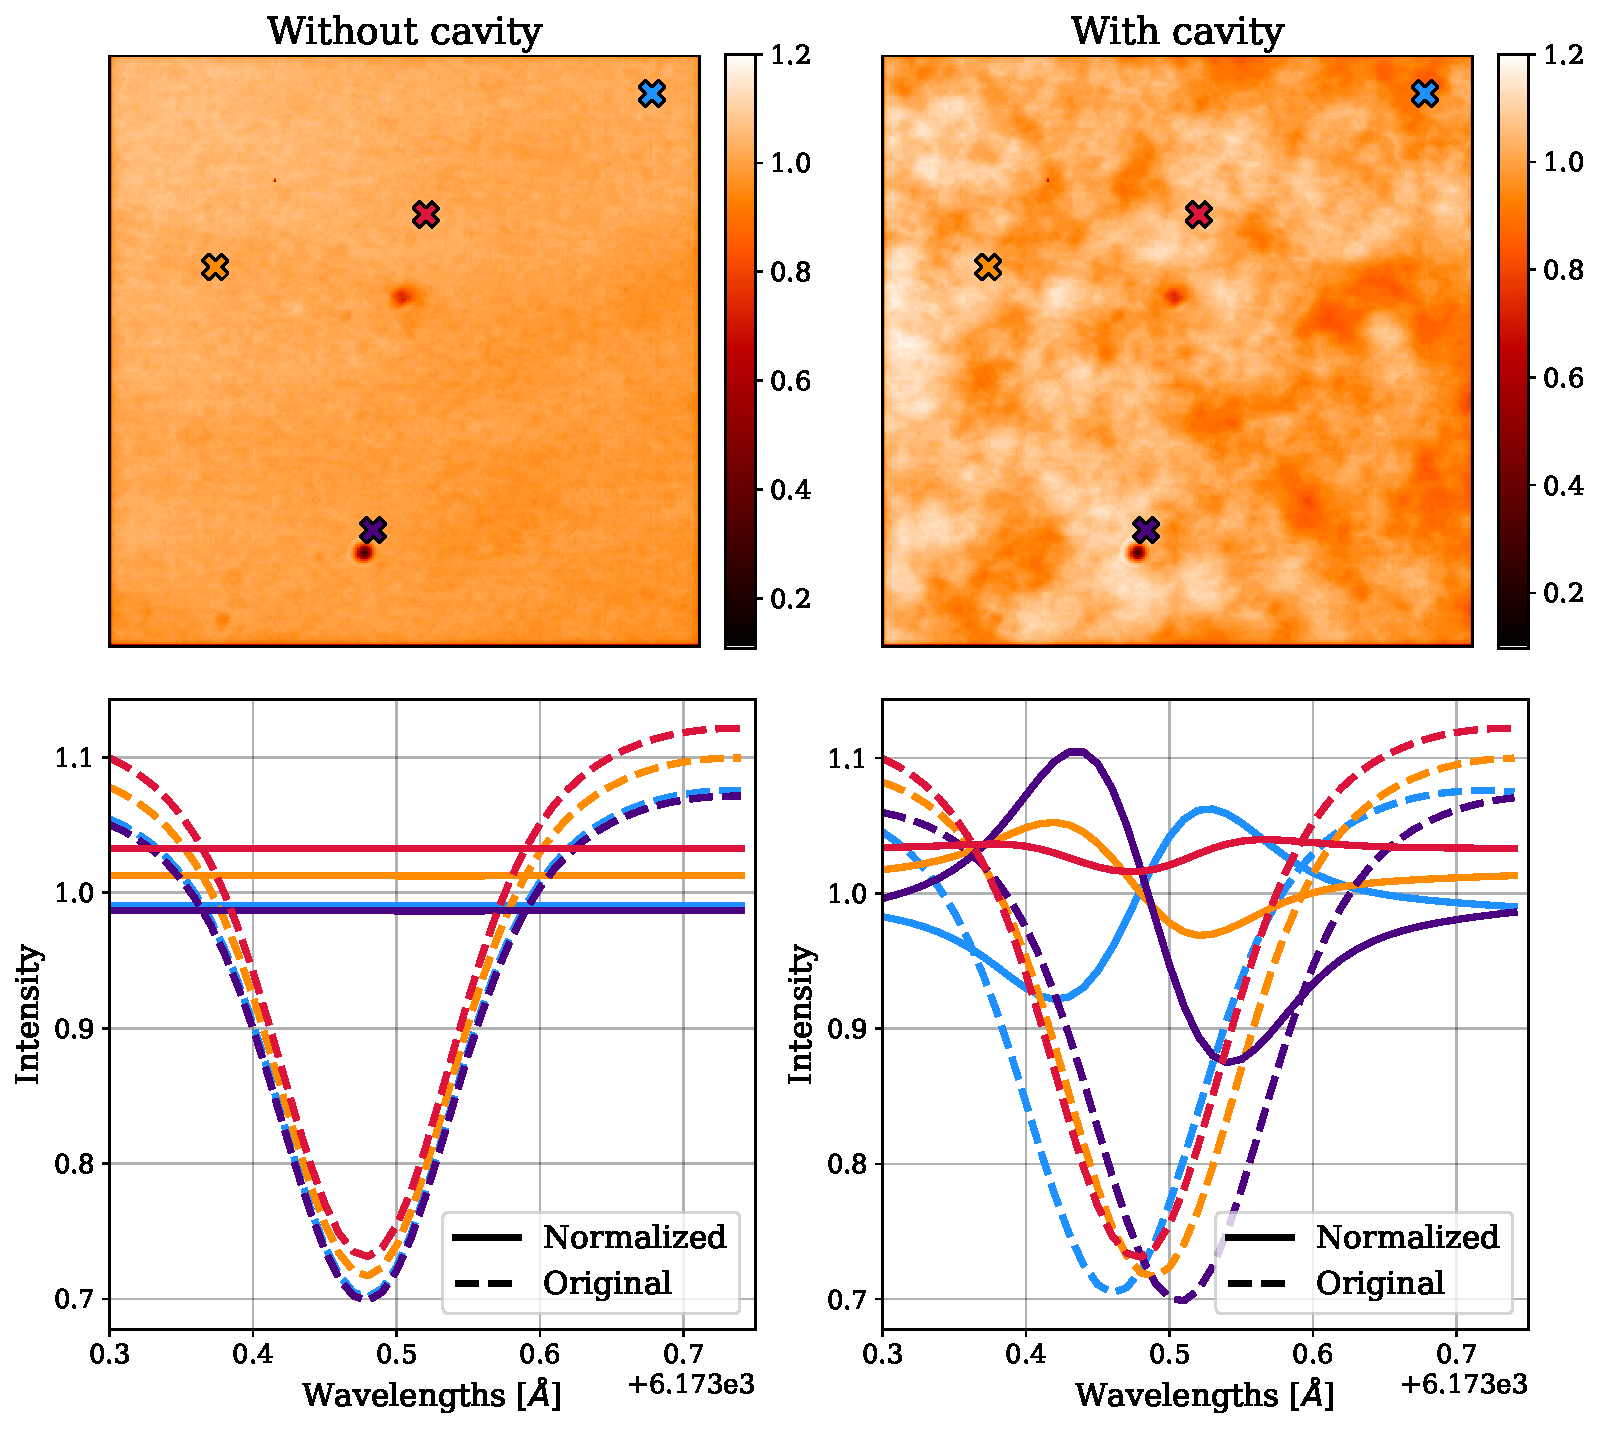
\includegraphics[width=\textwidth]{figures/Mancha/Flat_field_normalization.pdf}
  \end{minipage}\hfill
  \begin{minipage}[c]{0.27\textwidth}
    \caption[Flat-field profiles.]{
      The top row shows the observed flat-fields at the core of the line for both the simulations without (left) and with (right) cavity. The bottom row shows the spectral profile of the pixels marked with an "X" of the corresponding color, for both scenarios, and before and after the normalization.      
    \label{fig_mancha: flat_field normalization}} 
  \end{minipage}
\end{figure}

Figure \ref{fig_mancha: flat_field normalization} shows an image of the normalized flat-field at the line's core with and without taking into account the effects of the cavity map and the adverse effects it introduces when normalizing the flats to remove the spectral line. In the left panel one can clearly see the spatial structuring of the flat. Being constant for each wavelength (because it has no cavitssay effects) the normalization of the spectral lines (shown in the lower panel) is perfectly eliminated and the variation of the flat with wavelength is constant. However, the cavity map introduces a clear contamination in the flat during the normalization process. The intensity fluctuations that can be seen in the top right panel in fig \ref{fig_mancha: flat_field normalization} are due to the red and blue shift of the spectral line caused by the cavity map. The lower right panel shows the same profiles as in the non-cavity case. Again, the shifts due to the cavity map can be clearly seen. As we have explained before, normalizing the flat requires taking an intensity average at each wavelength. Since the flat shows imprints of the cavity, the normalized flat shows a clear intensity fluctuation on  wavelength. This dependence must exist, since one of the roles of the flat is to remove the etalon contribution, but since the etalon contribution is inside the integral in equation \eqref{eq_mancha: Intensity}, as we will see later, the flat is not able to entirely remove the effects of the cavity map. 

\begin{figure}
  \begin{minipage}[c]{0.7\textwidth}
    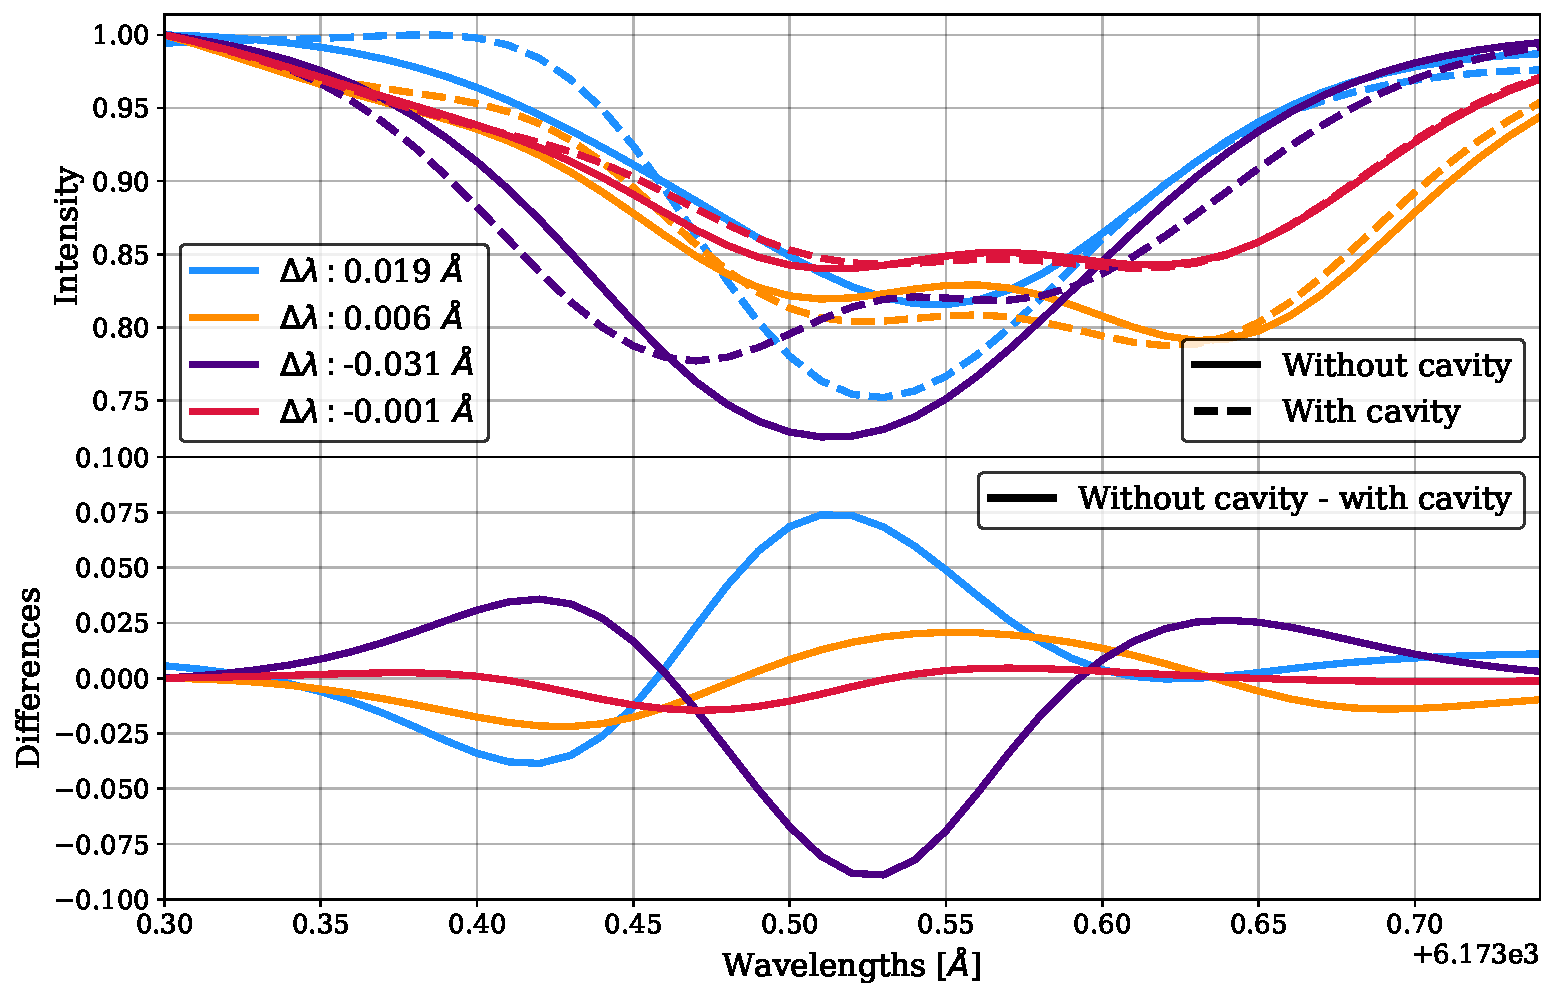
\includegraphics[width=\textwidth]{figures/Mancha/flatfield_norm_differences.pdf}
  \end{minipage}\hfill\hfill
  \begin{minipage}[c]{0.27\textwidth}
    \caption[Profiles after flat-field correction.]{
          The top panel shows four spectral profiles after the flat-field correction for the two scenarios, with and without cavity, and for the symmetric FPI. The selected pixels are the same than in Fig. ~\ref{fig_mancha: flat_field normalization}, and correspond to different values of the cavity map. The bottom panel shows the difference between the profiles with and witout cavities.
    \label{fig_mancha: Profiles_differences}} 
  \end{minipage}
\end{figure}

The issue with the flat-field correction is illustrated in Fig.~\ref{fig_mancha: Profiles_differences}, which displays the profiles after applying the correction for both scenarios, with and without the cavity map. Ideally, if the flat-field correction effectively compensates for the FPI cavity errors, the profiles from both scenarios should be identical. However, upon comparison, significant differences emerge, particularly for pixels with high cavity map values (light blue and dark blue lines). These profiles are not only shifted but also exhibit differences in their shape. 

Because of this, some data reduction pipelines adopt a different approach. Instead of using the flat-fields of the corresponding wavelengths, only the continuum flat-field is employed for the correction. When the continuum is measured sufficiently far from the spectral line, it remains unaffected by any spectral shift. By using this measurement, one can correct for spurious effects unrelated to spectral shifts, such as pixel sensitivity variations or dust grains. However, this method does not correct for the effects of the cavity.

If the cavity map is known, the velocity associated with the spectral shift caused by the cavity can be calculated. This "velocity-error" map can then be used to correct the Doppler velocity map derived from the observations that have not been corrected for the cavity map. This approach offers a partial solution, providing only a first-order approximation for correcting the spectral shift. However, it does not address the potential impacts of the cavity map on magnetic field calculations, as the relationship between wavelength shifts and magnetic fields is more complex than it is for velocity measurements.

\subsection{\label{sect: mancha_vlos}Velocity maps}

We begin our analysis by studying the LOS velocities and the errors associated with their computation. These velocities are derived from the spectral shift of each profile relative to the rest position of the spectral line, using the Doppler formula, eq.~\eqref{eq_spectro: Doppler}. Given that this computation relies exclusively on the spectral shift, it is particularly susceptible to errors caused by cavity effects.

According to the center-of-gravity method \citep{center_of_gravity}, the central wavelength of a given spectral profile, $\lambda _ {COG}$, can be computed from:

\begin{equation}
  \lambda _ {COG} = \frac{\int \lambda \left( I _{cont} - I\right)d\lambda}{\int \left( I _{cont} - I\right)d\lambda}. 
\end{equation}

Once $\lambda _ {COG}$ has been determined, the spectral shift of the corresponding profile will be given by $\Delta \lambda = \lambda _ 0 - \lambda _ {COG}$. 

We have computed the velocities employing the two flat-field correction strategies mentioned in the previous section: the "standard" approach, where each observation is corrected with the flat-field of the corresponding wavelength; and the "continuum" approach, where only the continuum flat-field is employed. The top row of figure \ref{fig_mancha: int_and_vlos_examples} shows the continuum intensity and the velocity maps obtained for both strategies.  

\begin{figure}[t]
  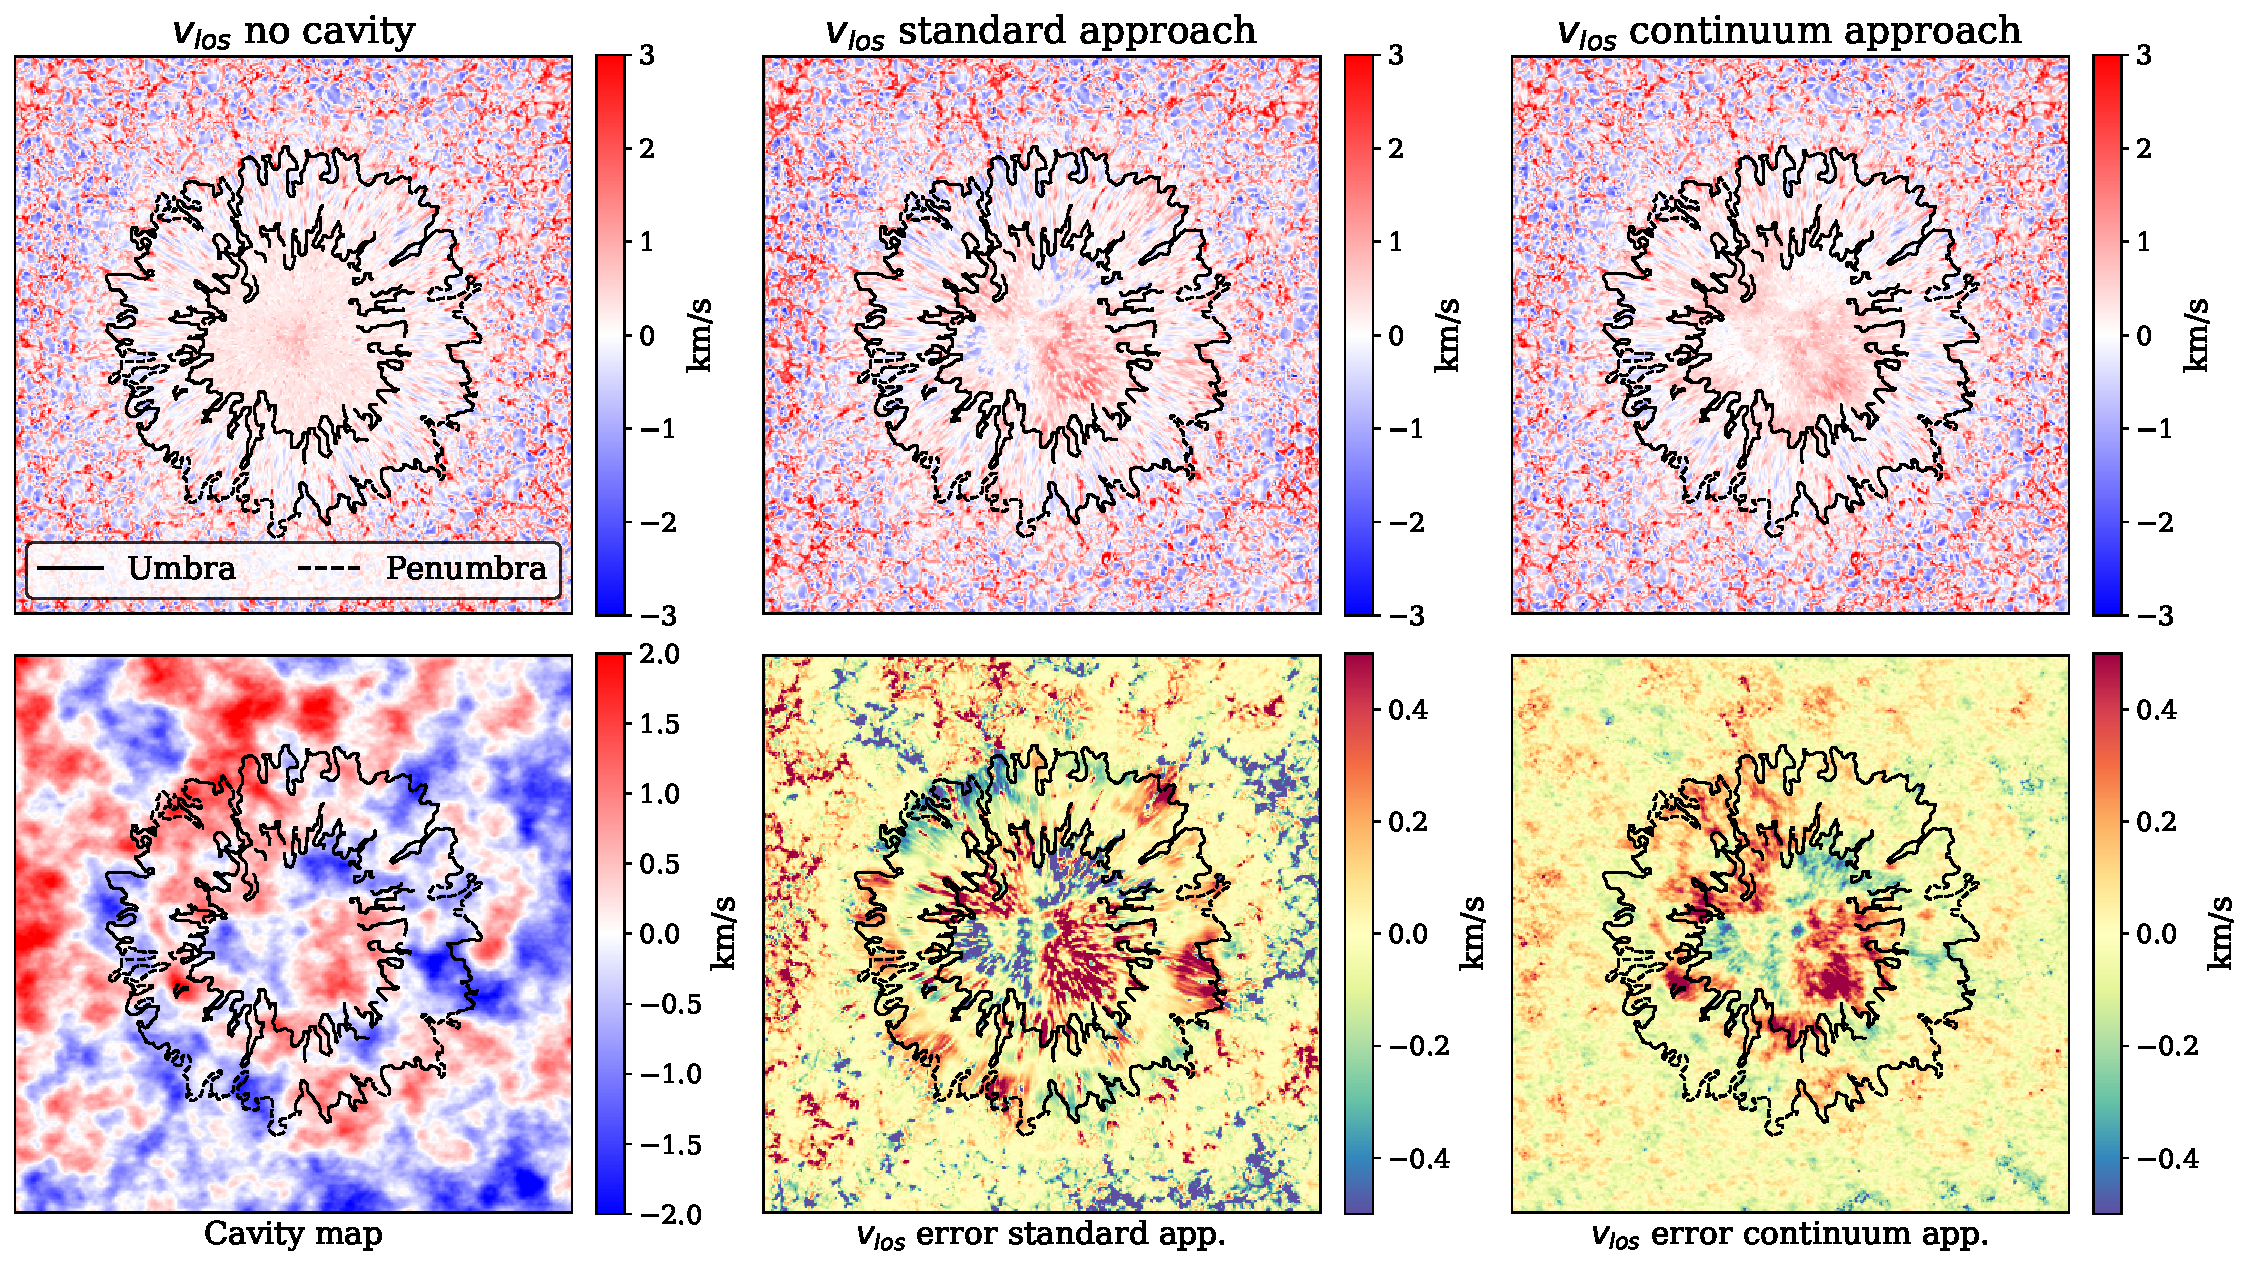
\includegraphics[width=\textwidth]{figures/Mancha/intensity_and_vlos_examples.pdf}
  \caption[Sunspot velocity errors.]{
    The top row shows, from left to right, the observed intensity in the continuum, the LOS velocity for the standard approach and the LOS velocity for the continuum approach, all three for the symmetric FPI and belonging to the simulations with cavity map. The bottom row shows, from left to right, the velocity error associated with the cavity map, the error for the LOS velocity for the standard approach and the error for the LOS velocity of the continuum approach. The error is computed by substracting the measurement to the reference. All representations show the boundaries of the umbra and penumbra for an easier identification of the regions in the velocity and cavity maps.   
    \label{fig_mancha: int_and_vlos_examples}}
\end{figure}

At first glance, the velocities derived for each approach look qualitatively similar, but under closer inspection, some differences exist. In order to highlight these differences and to assess their accuracy we will compare them to the velocity obtained in the scenario where no cavity map was introduced. Figure \ref{fig_mancha: int_and_vlos_examples} shows this comparisons in the bottom row, along with the cavity map with the umbra and penumbra boundaries overplotted for comparison purposes.

The error in the velocity computation shows that the effects of the cavity map remain uncorrected in the observations. Both correction approaches exhibit errors with structures corresponding to the cavity map. For the standard correction, this effect is pervasive throughout the field of view (FoV), whereas for the continuum approach, it is primarily concentrated in the umbra, although other regions also exhibit this behavior.

Moreover, the errors are significant, given that regions of the penumbra show errors of around 10\%. Errors in the umbra are similarly significant in percentage terms, if not worse; however, studies of these regions are less frequent due to their low S/N resulting from their inherent darkness. Conversely, as discussed in the introduction, penumbral flows are of particular interest, prompting us to prioritize our discussion on the results in that area. Outside the umbra, the velocities are generally underestimated for pixels affected from a blueshift displacement due to the cavity, and overestimated for redshifts, resulting in an error pattern that follows that of the cavity map. The general performance of the correction is worse when employing the standard approach versus the continuum strategy. Except for the umbra, where this behavior is reversed.     

\begin{figure}
  \begin{minipage}[c]{0.7\textwidth}
    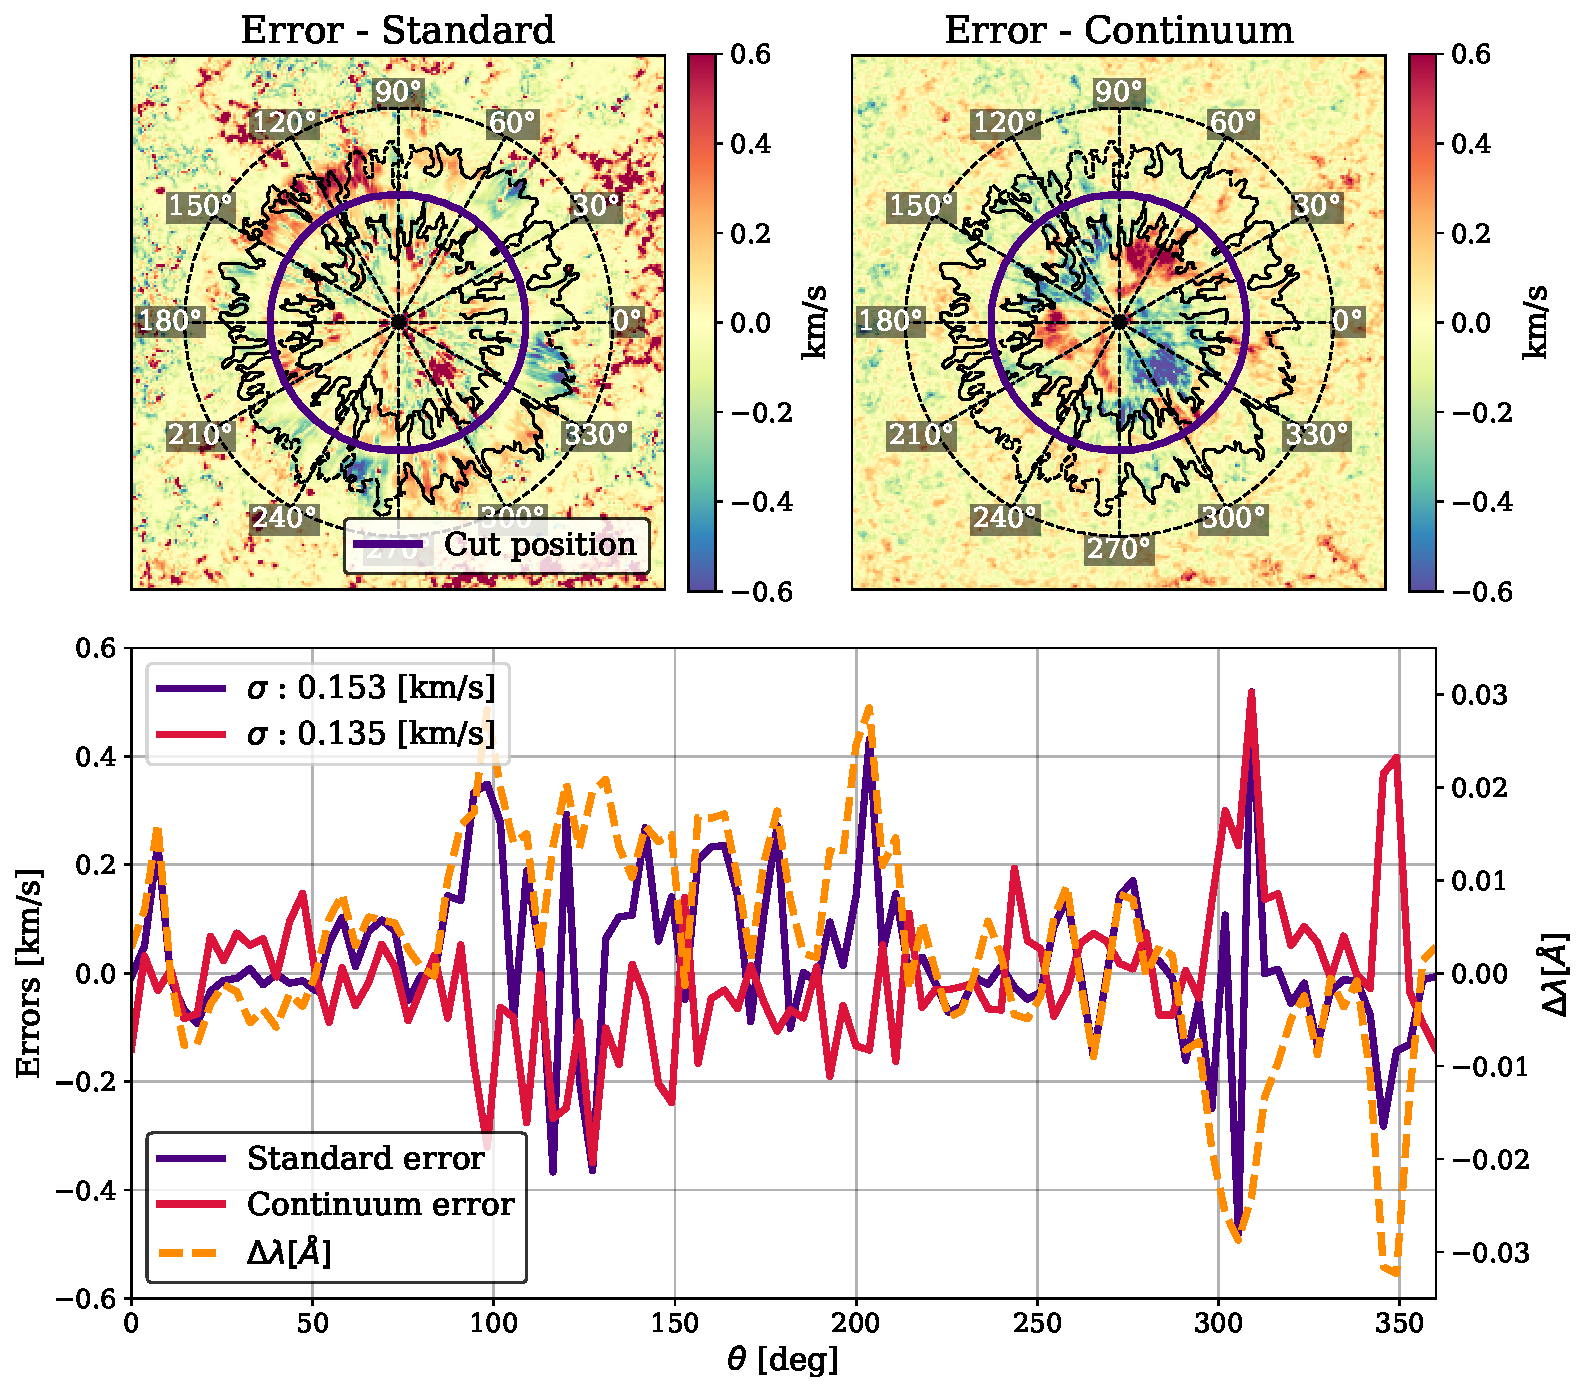
\includegraphics[width=\textwidth]{figures/Mancha/circular_cut_standard_cont.pdf}
  \end{minipage}\hfill\hfill
  \begin{minipage}[c]{0.27\textwidth}
    \caption[Velocity error, radial cut.]{
      The top row shows the velocity error maps for both the standard and continuum approaches, along with the cut position and an overlay of the degrees for easier interpretation of the plotted profiles. The bottom panel shows the velocities along the cut for both aproaches along with the value of the cavity map at the corresponding position.\label{fig_mancha: verror_circular_cut}} 
  \end{minipage}
\end{figure}

A more quantitative analysis is shown in Fig. \ref{fig_mancha: verror_circular_cut}, where the velocity error along a circular path is shown, for both approaches, in addition to the associated spectral shift of the cavity values at identical positions. In the figure it can be seen how there is no strong correlation between the cavity map and the errors in the velocities in both cases, taking into account all wavelengths or only the continuum. In the first case, there is some correlation but it is not significant.

Some pipelines address cavity-map issues by attempting to "deconvolve" the etalon's transmission profile from the flat-field observations. However, it is common practice to overlook the asymmetric nature of real telecentric mounts due to the complexity of the analytical equations involved, and because the potential effects of profile asymmetries are often assumed to be negligible.


\begin{figure}
  \begin{minipage}[c]{0.5\textwidth}
    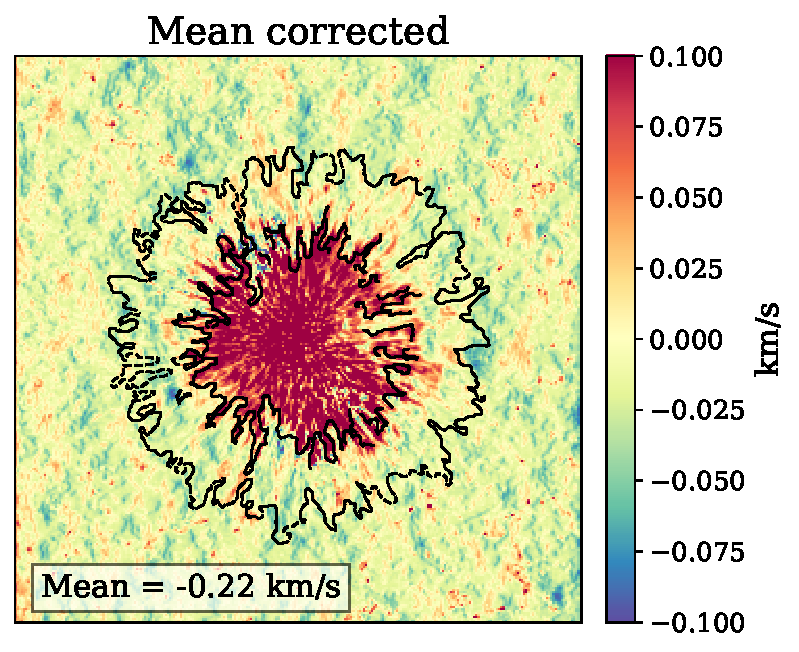
\includegraphics[width=\textwidth]{figures/Mancha/vlos_sym_vs_asym.pdf}
  \end{minipage}\hfill\hfill
  \begin{minipage}[c]{0.47\textwidth}
    \caption[Assymetry effect in velocity calculations.]{
      Difference in LOS velocities between the symmetric and assymetric FPIs (symmetric - asymmetric). The mean value of the difference has been substracted for the whole FoV. \label{fig_mancha: vlos_asym_vs_sym}} 
  \end{minipage}
\end{figure}

In an attempt to quantify the error of this assumptions, we now compare the results obtained with the asymmetric and symmetric profiles. The main effect of the asymmetry is a systematic shift of the profile measurements towards the blue. This shift results in an average difference of around $-0.2$ km s$^{-1}$ that can be seen over the whole FoV. 

Nevertheless, this systematic shift can be removed from the velocities computed with the asymmetric FPI by substracting the average difference between symmetric and asymmetric velocities. Figure \ref{fig_mancha: vlos_asym_vs_sym} depicts the differences in the computed velocities for the symmetric and asymmetric FPIs, after applying this correction. Despite accounting for the systematic shift, discrepancies are still present, predominantly within the umbra, although they are observed across the entire FoV. The umbra is again more sensible than other regions, with velocity discrepancies higher than 100 m s$^{-1}$ throughout the majority of the umbra, and exhibiting a global shift towards smaller velocities for the asymmetric scenario. Outside the umbra, differences are smaller but still prevalent throughout the entire FoV. 

The fact that the umbra exhibits different behaviors compared to the rest of the FoV, along with the difference between the two types of FPIs, suggests that the amplitude and behavior of these effects are very sensitive to the shape of the observed spectral profile and the FPI's transmission profile, as expected from the dependence observed in the equations (see. eq.\eqref{eq_mancha: Intensity}).  

\subsection{\label{sect: mancha_blos}Magnetic field maps.}

It is expected that cavity errors significantly impact velocity calculations, as these are derived solely from the analysis of spectral shifts. However, the effect of these errors on the calculation of the magnetic field is not as straightforward as its determination involves not only the spectroscopy, but also polarization. 

To calculate $B_{LOS}$, we need to determine the circularly polarized component of the light. This requires demodulating the simulated observation using a process analogous to that described in the TuMag pipeline. Once the Stokes components have been determined, the LOS component of the magnetic field is computed using the center-of-gravity method  (eq.~\eqref{eq_spectro: Blos-cog}). 

\begin{figure}
  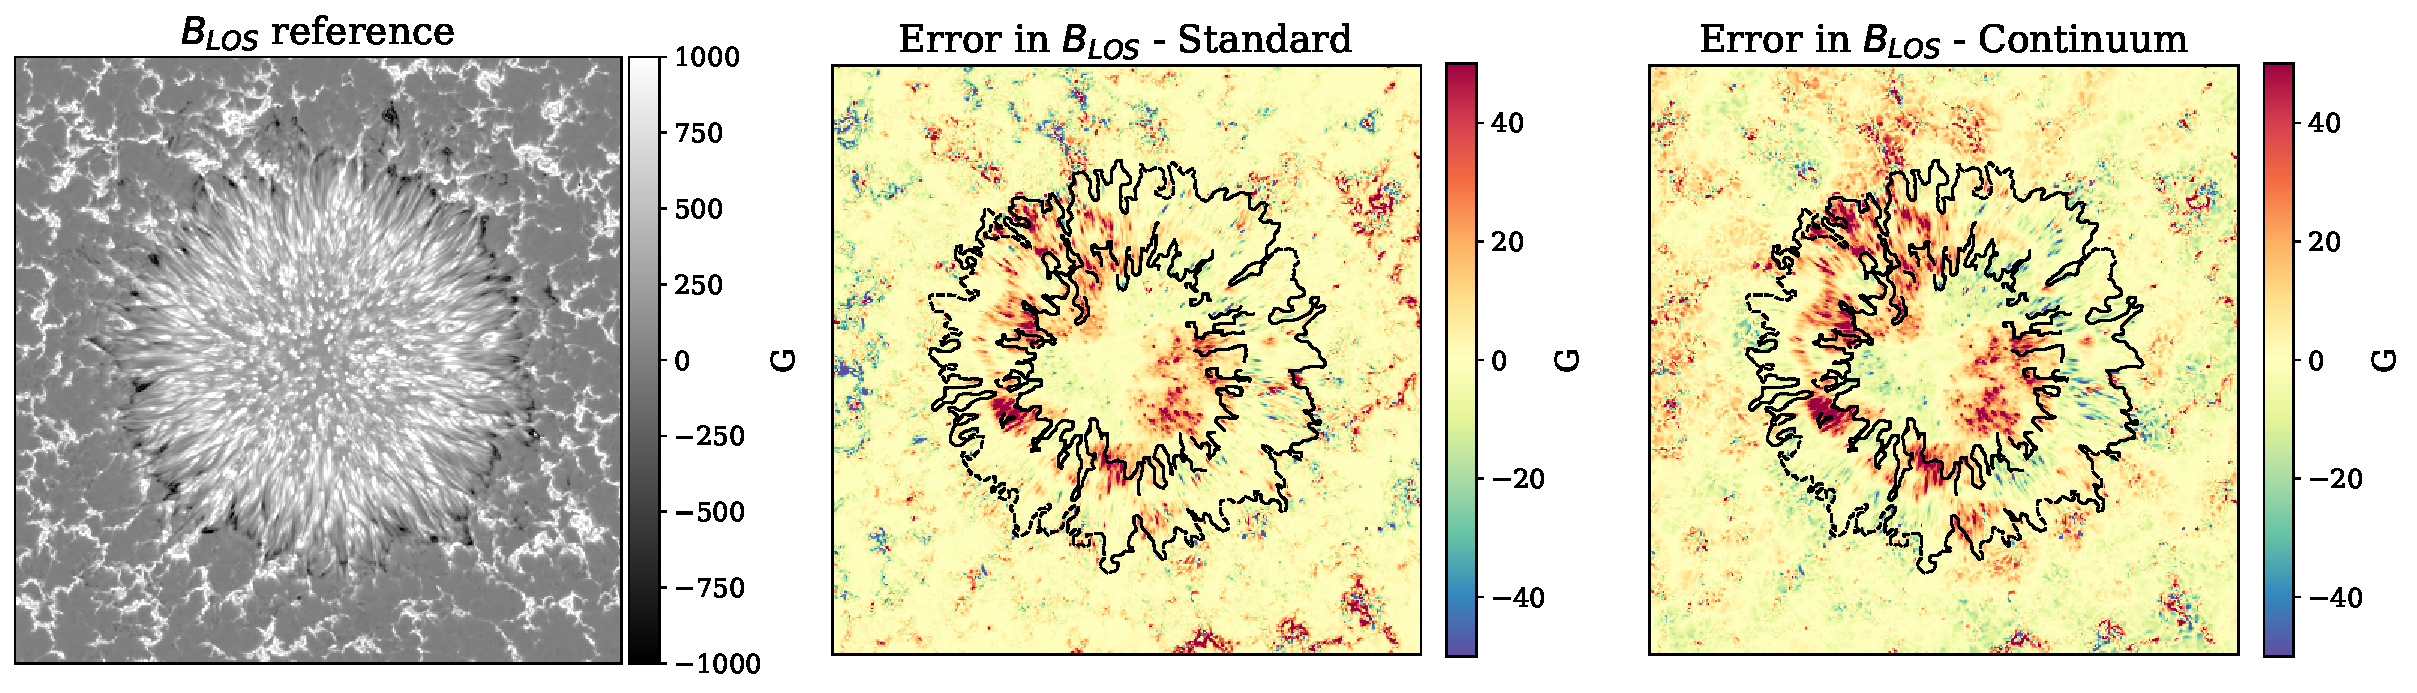
\includegraphics[width=\textwidth]{figures/Mancha/blos_errors.pdf}
  \caption[Error in Blos calculation.]{
    From left to right, $B_{LOS}$ for the simulation with no cavity and a symmetric FPI, error in $B_{LOS}$ computation for the standard approach with a symmetric FPI, and error in $B_{LOS}$ computation for the continuum approach with a symmetric FPI. 
    \label{fig_mancha: blos_errors}}
\end{figure}

Figure \ref{fig_mancha: blos_errors} shows the LOS component of the magnetic field for the simulation with no cavity (the one employed as reference) and the errors in its calculation for both flat-fielding approaches.  In the continuum approach, the structures observed in the error map closely resemble those in the cavity map. This similarity is expected since no correction has been applied to account for the cavity error. While it is possible to compute the velocities associated with the spectral shift caused by the cavity map, this is not feasible for the magnetic field. Consequently, any effect of the cavity remains in the data when using the continuum approach.

As a result, errors in the magnetic field computation appear larger or more prevalent across the entire field of view (FoV) for the continuum approach. However, for both correction strategies, the errors remain relatively small, reaching values of approximately 3 G, compared to magnetic field signals of around $\pm 100$ G. Although small, these residuals of the cavity map in the magnetic field maps are one of the main problems of employing the continuum approach in real data.

\section{\label{sect: etalon_corr_fitting}Fitting algorithm}

Results from the sunspot observation simulation highlight the relevance of carefully addressing the data correction of FPI-based instruments. Although some pipelines address these deviations by correcting them only at first order through a regular flat-fielding procedure with no further computations, the residues left in the data can lead to errors as high as those shown in the previous section, depending on the FPI's properties. For this reason, different approaches have been taken to address these additional corrections. Typically, each instrument has a specific data reduction pipeline where the corrections are carried out taking into account the individual properties of the instruments, hence giving rise to different methods. An example of a more detailed calibration pipeline can be found in \cite{crisp-method}. By using a simplified analytical expression for the etalon transmission profile, Schnerr et al. were able to extract from the flat fields the contributions caused by the FPI cavity errors and variations in reflectivity for the CRISP instrument, which are then taken into account in the data calibration.

For the first order, this is a good approximation, but since asymmetries in the transmission profiles naturally arise in telecentric instruments \citep{franI}, deviations originating from them cannot be fully corrected. Thus, knowledge of the exact shape of the transmission profile is necessary to fully account for these deviations. \cite{schamer_method} already allowed asymmetries to be dealt with in the pipeline of the CRISP instrument, but the asymmetries originated from wavelength shifts induced by two distinct etalons, or from an angular dependence along the FoV introduced to approximate the behavior in telecentric setups.  

We aim to further extend and generalize the strategy employed in \cite{crisp-method} and \cite{schamer_method} by including the exact shape of the transmission profile for the telecentric configuration in the analysis. By doing so, we can fit and take into account the presence of asymmetries in the profile that arise in these setups due to an asymmetric pupil apodization. We have developed a method for deriving the etalon properties from the data in such a way that prior knowledge of the distribution and magnitude of the defects is not needed. We do not make any distinction between defects associated with the mirror's flatness or separation, refraction index, or cavities. This way, we ensure the applicability of the algorithm to all types of FPIs (air and solid). Our technique also differentiates the effects associated with the etalon from other corrections not related to it, such as pixel-to-pixel variations of the gain across the detector. By comparing the theoretical prediction, obtained through the analytical expressions of the transmission profile, with the measured data, we can disentangle the etalon properties from the flat-field observations. 

In this section, we introduce the algorithm and evaluate its performance. We begin by outlining the approximations made and detailing the algorithm in Sections \ref{eta_corr_susec: approx and simulations} and \ref{eta_corr_susec: fitting algorithm}, respectively. The method was tested on a series of simulated observations with controlled configurations to evaluate the impact of different observational properties on the accuracy of the results. Finally, the algorithm was applied to a dataset from the HRT telescope of the SO/PHI instrument to assess its performance in real scenarios. The results for both the simulated scenarios and real data are discussed in Section \ref{eta_corr_susec: results}.

\subsection{\label{eta_corr_susec: approx and simulations}Initial approximations and observations simulation.}

As initial approximations, we will adopt the same assumption regarding the prefilter as the one employed for the sunspot simulation; specifically, that it has a rectangular shape with a width such that only one order of the etalon is let through. Additionally, we will disregard the spatial PSF of the FPI and assume that the spatial dependence can be represented by a Dirac delta function to simplify the equations. Therefore, if we assume that the image response of the FPI follows the expression:
\begin{equation}
S\left(\xi_0, \eta_0; \xi , \eta; \lambda-\lambda_{s}\right)=\delta(\xi_0-\xi,\eta_0-\eta)\Psi(\xi,\eta,\lambda-\lambda_s),
\end{equation}
equation \eqref{eq_mancha: Intensity} simplifies into:
\begin{equation}
    I\left(\xi, \eta ; \lambda_{s}\right)=g(\xi, \eta)\int_{\lambda _ 0 - \Delta \lambda}^{\lambda _ 0 + \Delta \lambda} O\left(\xi, \eta ; \lambda\right) \Psi\left(\xi, \eta ; \lambda-\lambda_{s}\right)  \mathrm{d} \lambda.
    \label{eq_eta_corr: intensity}
\end{equation}

The explicit shape of $\Psi$ varies depending on the optical configuration of the instrument, whether collimated or telecentric. In particular, we will employ three types of transmission profiles: one for the collimated configuration, one for a perfect telecentric setup (normal incidence), and one for an imperfect telecentric setup. The first two have analytical expressions for the transmission profile in the absence of the spatial PSF, as detailed in Sections \ref{susec_etalon_theory: collimated} and \ref{susec_etalon_theory: Tele-perfe}, respectively. For the imperfect telecentric configuration, the transmission profile must be determined numerically (see Section \ref{etalon_theory: Tele-imperfe}).
  
We have tested the performance of the algorithm on a series of simulations of a spectral line observation in different conditions. We used the Kitt Peak FTS-Spectral-Atlas as the reference \citep{fts} and, specifically, the Fe I spectral line at 6173.3~\r{A}. Each observation was composed of $N_\lambda$ wavelengths, where the measured intensity was recorded. At every wavelength $\lambda_s$, the corresponding transmission profile of the etalon $\Psi^{\lambda_s}$ was computed, and the "observed" intensity $I ^{\lambda _ s} _ {{\rm obs}, i}$ corresponding to a specific spatial location $(\xi, \eta)$, represented hereinafter by the pixel $i$, was calculated using Eq.~\eqref{eq_eta_corr: intensity}. Additionally, we took into account the presence of additive Gaussian noise. This noise does not necessarily respond to any parameter fluctuation within our analytical expressions or photon noise but comes from any unexpected variations that may not have been modeled in the theoretical scheme.

Additionally, we included the presence of defects arising from irregularities or inhomogeneities on either the cavity thickness $d$, the refractive index $n$, or from deviations of the angle of incidence $\theta$. In order to simulate this, we introduced a relative perturbation $\Delta a$ into the etalon equation that accounts for any local deviation of the value of $a$ with respect to its nominal value. This parameter changes from pixel to pixel differently for the collimated and telecentric configurations. In the former, the profile shifts across the FoV only because of the different incidence angles of the light beam on the etalon. In the latter, local variations of $n$ and/or $d$ are mapped directly onto the detector. We also note that variations in the incidence angle must be considered as well when the degree of telecentrism varies along the detector. Analytically, the parameter $a$ at each $i$-th pixel is given by $a' _ i = a \Delta a _ i$, where $a = (2\pi/\lambda) n d\cos\theta$ is constant along the FoV. Note that rewriting the equations for the transmission profiles (sections \ref{susec_etalon_theory: collimated} and \ref{susec_etalon_theory: Tele-perfe}) using this definition of $a$ is straightforward. In collimated configurations, the parameter $\delta$ (eq. \eqref{eq_etalon_theory: collimated_delta}) is simply $2a$. In perfect telecentric configurations, $\theta$ is always 0, so the given transmission profile is already expressed in terms of $a$.   

We let $n _ i ^{\lambda_s}$ be the  noise contribution at the $i$-th pixel and wavelength $\lambda_s$. Thus, the observed intensity at that pixel when the etalon is tuned at $\lambda _s$, $I ^{\lambda _ s} _ {{\rm obs}, i}$ is given by 
\begin{equation}
I ^{\lambda _ s} _ {{\rm obs}, i} = g_i \frac{\int_{\lambda_0 - \Delta \lambda}^{\lambda_0 + \Delta \lambda} O(\lambda)\Psi^{\lambda _ s} (\lambda , \Delta a _i)  d\lambda}{\int_{\lambda_0 - \Delta \lambda}^{\lambda_0 + \Delta \lambda} O(\lambda)\Psi^{\lambda _ c} (\lambda, \Delta a _ i)  d\lambda} + n _ i ^{\lambda_s}    ,
\label{eq_eta_corr: Profile - General}
\end{equation}
with $\lambda _ c$ being the continuum wavelength. From a practical point of view, the integration limits are set in such a way that only a single resonance (or order) of the etalon is included with the limits, thus, acting akin to the sorting pre-filter commented on previously. We note that the denominator strictly corresponds to the intensity at the continuum of the line in the absence of the transmission profile or if the continuum wavelength is far enough from the spectral line. In any other case, the transmission should be taken into account as well to normalize the observations to the local continuum, which is necessary since we work with relative measurements. An example of a spectral line measurement is displayed in Fig.~\ref{fig_etalon_corr: Prof-Measure}.
\begin{figure}
    \centering
    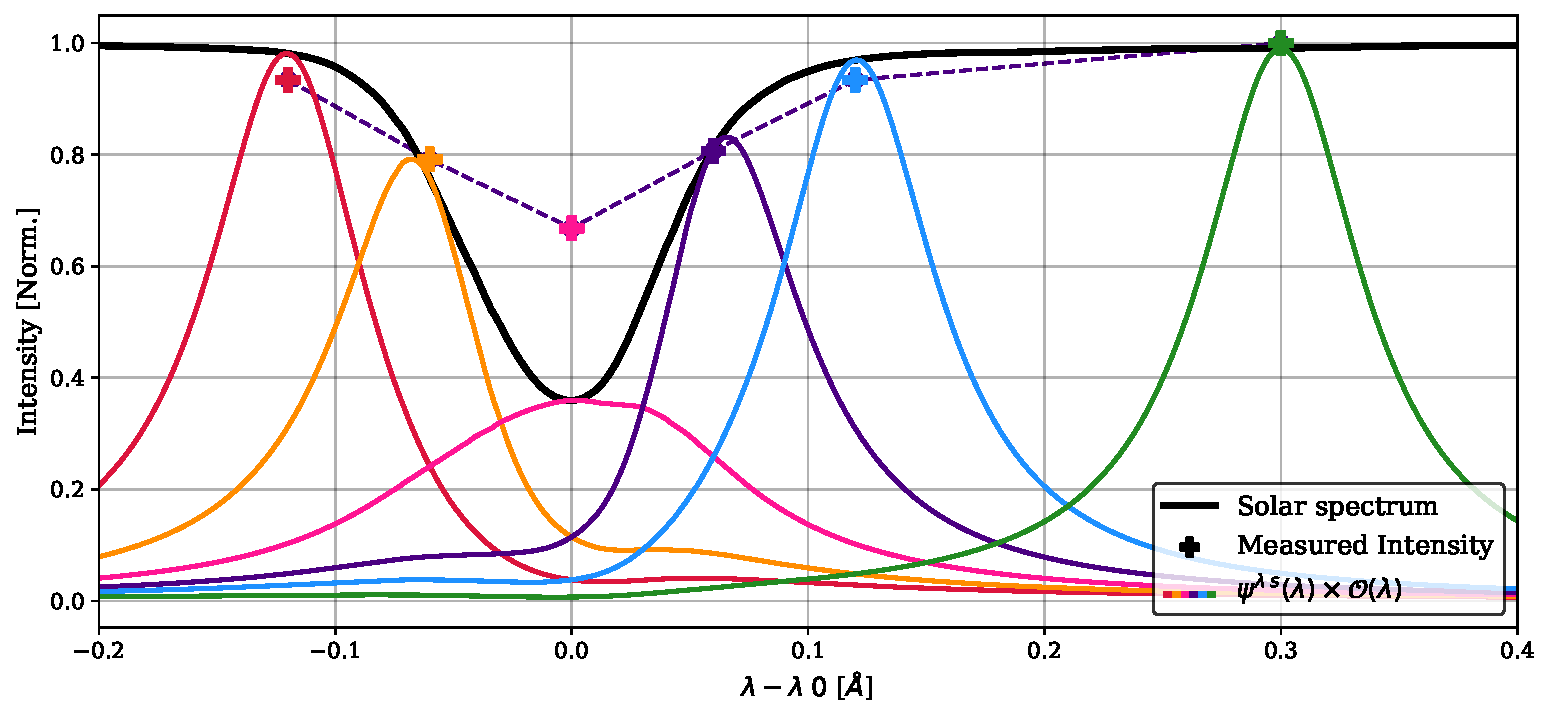
\includegraphics[width = \textwidth]{figures/EtalonPaper/ProfileMeasurement.pdf}
    \caption[Simulation of a spectral line scan.]{Simulated observation of the Fe I spectral line ($\lambda _ 0 = 6173.3$\r{A}) using a collimated mount and a total of $N_ \lambda = 6$ wavelengths that have been equally distributed along the spectral line, with the exception of the continuum measurement (light blue), which is selected at $300$ m\r{A} from the blue of the line core. The measured intensity is the result of computing the value given by Eq.~\ref{eq_eta_corr: Profile - General} at each wavelength and with $g = 1$.
    } \label{fig_etalon_corr: Prof-Measure}
\end{figure}

For both the collimated and telecentric configurations, we modeled etalon and gain imperfections over a $100\times100$~px$^2$ image. Pixel-to-pixel variations in the sensor efficiency were modeled following a random spatial distribution, as shown in Fig.~ \ref{fig_etalon_corr: Inputs} (left panel). Additionally, we included a set of pixels with very low gain values, which represent a group of dead pixels or dust grains.

We modeled the etalon defects as changes in $\Delta a$ in such a way that the maximum displacement reaches $3$ pm. The spatial distribution of the values of  $\Delta a $ follows an increasing radial distribution, as shown in Fig.~ \ref{fig_etalon_corr: Inputs} (right panel). Such a spatial distribution coincides with the expected one in collimated etalons due to the change in the incidence angle across the FoV. Telecentric mounts do not exhibit a spatial distribution of their defects such as this, but using the same spatial distribution in the two cases allowed us to compare the performance of the method for both setups in a systematic way. Since $\Delta a$ accounts for relative perturbations, it is by definition an adimensional parameter. However, to grant it a physical meaning, we express the values of $\Delta a$ in \r{A}, representing the associated shift of the transmission profile with respect to the original position determined by $a$.

\begin{figure}[t]
  \centering
    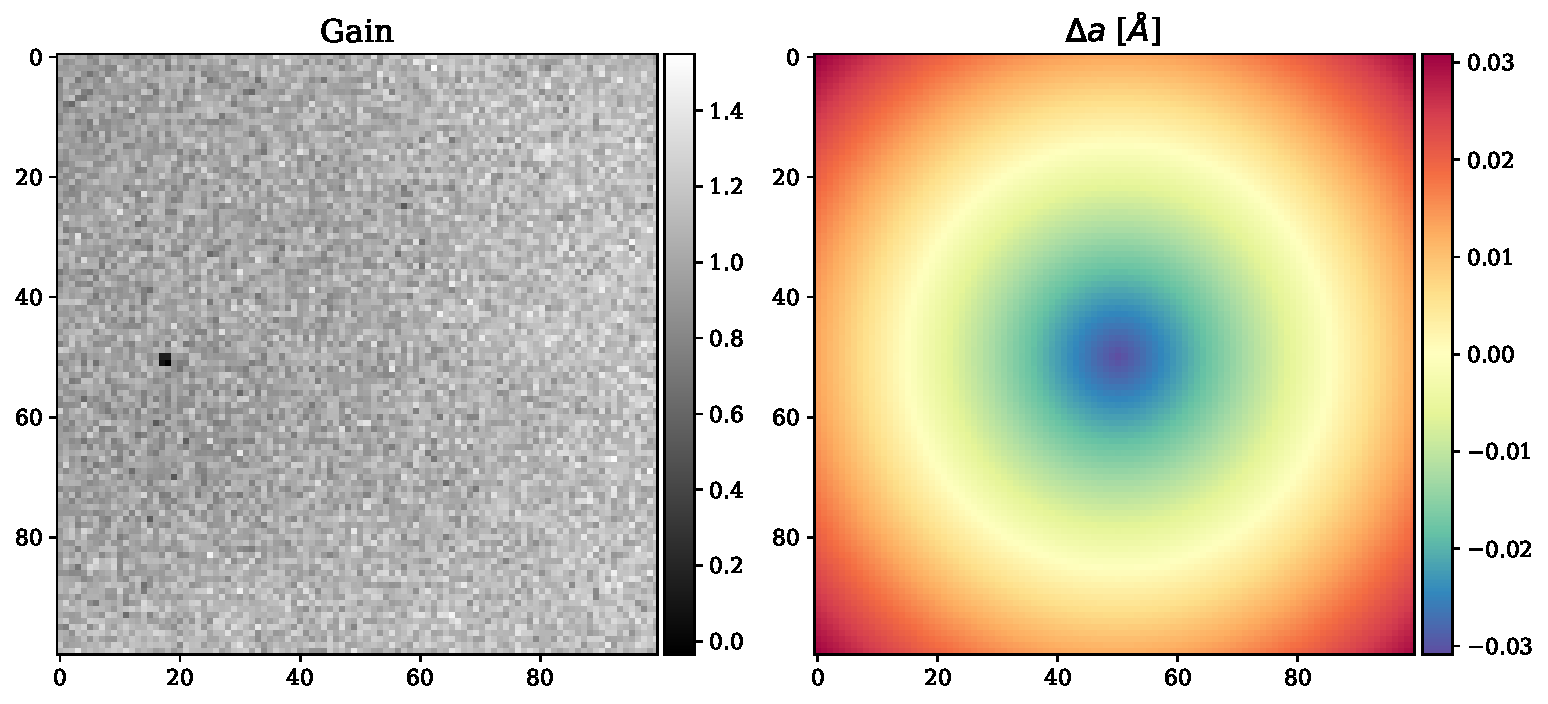
\includegraphics[width=\textwidth]{figures/EtalonPaper/Gain_Da_Inputs.pdf}
    \caption[Simulation inputs.]{
      Input maps introduced when simulating the observations. The left panel represents the gain generated as white Gaussian noise, with values ranging from 0.8 to 1.2. A dust speck was introduced by creating a group of four pixels with low values of $g=0.2$ for the gain. The right panel shows the spatial distribution of the defects in the etalon. The distribution follows a radial pattern starting from the center of the FoV. The defects vary from $0\,\%$ deviation to up to $5\times 10 ^{-4}\,\%$, which corresponds to a shift of 3~pm. Both possible directions for the deviations have been considered. The sign of the deviation is negative at the very center, which introduces a redshift, while it is positive at the corners, causing a shift of the profile into the blue.
      \label{fig_etalon_corr: Inputs}}
\end{figure}

\subsection{\label{eta_corr_susec: fitting algorithm}Fitting algorithm}

We have developed an algorithm able to extract the distribution of the etalon defects and the gain map from data taken by etalon-based instruments, which enables the correction of the two contributions separately. The algorithm works by minimizing a given merit function that depends on the gain and the etalon defects. 

In particular, we have defined an error metric, $\varepsilon  ^\lambda$, at each tuned wavelength, computed by comparing the measured intensity with the theoretical prediction. If we let $I_ {i, {\rm obs}} ^{\lambda _s}$ be the measured intensity at a given $i$ pixel for an etalon tuned to the wavelength $\lambda_s$, the error metric at each wavelength is given by
\begin{equation}
\varepsilon ^{\lambda _s} (\Delta a _i, g _ i) =  I _ {i, {\rm obs}} ^{\lambda _ s} - g_i \frac{\int_{\lambda_p}^{\lambda_q} O(\lambda)\Psi^{\lambda _ s} (\lambda, \Delta a _ i)  d\lambda}{\int_{\lambda_p}^{\lambda_q} O(\lambda)\Psi^{\lambda _ c} (\lambda, \Delta a _ i)  d\lambda}
\label{eq_eta_corr: Error metric}.
\end{equation}

The merit function we employed is then the quadratic summation of the error metric over all tuned wavelengths:

\begin{equation}
f(\Delta a _i, g _ i) = \sum _ {s = 0} ^ {N_\lambda} \left( \varepsilon ^{\lambda _s} (\Delta a _i, g _ i) \right) ^ 2.  
\label{eq_eta_corr: Merit Function}
\end{equation}
Both the camera gain and the defects of the etalon change from one pixel to another, which is why we address each pixel independently, but they remain constant at every wavelength. Hence, the transmission profile of the etalon varies at different points of the FoV; but at a given pixel, it is constant at all tuned wavelengths. Therefore, the algorithm is able to better obtain the etalon properties as we increase the number of wavelengths.

Figure \ref{fig_etalon_corr: Derivatives} shows the derivatives of the error metric, Eq.~\eqref{eq_eta_corr: Error metric}, as a function of wavelength, that is, before computing the summation over $s$ of the merit function, with respect to the gain, the reflectivity, and $\Delta $a. The curve corresponding to the $\Delta a$ derivative is different from the others, whereas the derivatives of both the gain and the reflectivity exhibit similar shapes. Hence, variations in either the reflectivity or the gain introduce similar changes in the merit function, which can produce a trade-off between these two parameters, especially when the spectral line is sampled in only a few points. Given that discrepancies arising from errors in reflectivity are assimilated by gain maps, we did not take into account reflectivity errors when computing our simulations, as they have no impact on cavity map calculations.

\begin{figure}
  \begin{minipage}[c]{0.6\textwidth}
    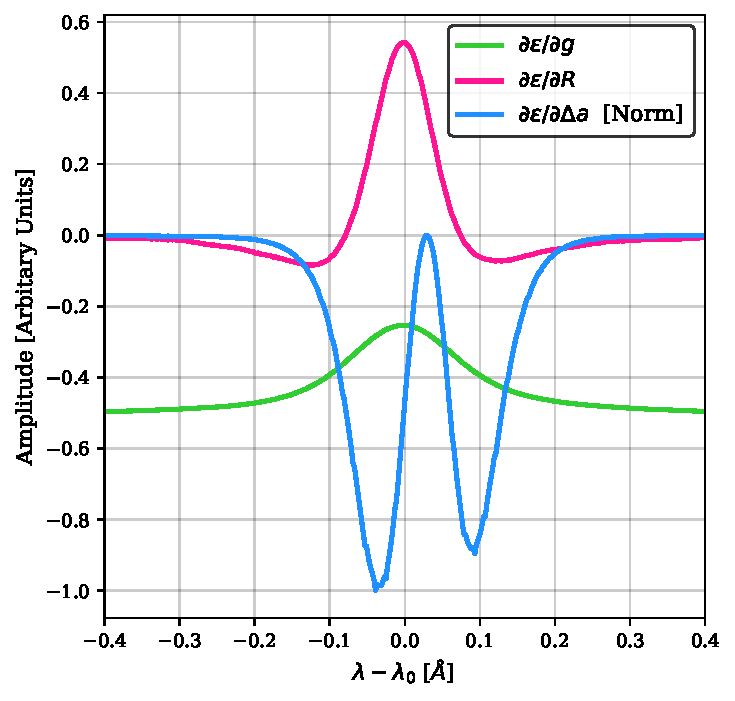
\includegraphics[width=\textwidth]{figures/EtalonPaper/Derivadas.pdf}
  \end{minipage}\hfill
  \begin{minipage}[c]{0.37\textwidth}
    \caption[Derivatives of metrit function]{
      Derivatives of the error metric as a function of wavelength. The derivative with respect to $\Delta a$ has been normalized in order to fit the three curves in the same plot. \label{fig_etalon_corr: Derivatives}} 
  \end{minipage}
\end{figure}


A few key aspects arise when analyzing the merit function and its applicability on real data. The first point to bear in mind is that the shape of the object, $O(\lambda)$, is not known a priory. Therefore, we needed to provide a guess for it. The method works by assuming that differences between the prediction and the observation are caused exclusively by the etalon defects or the gain. If the object used during the fitting process differs considerably from the real one, the prediction and observation will have differences that will erroneously be identified as etalon defects or gain variations. This is the main source of errors for the method when applied to real data. Two approaches can be followed in order to address this issue. The first one consists of assuming the solar atlas profile as the object. This is a good approximation, provided the data to which the algorithm is applied to lack information about solar structure, either because they are observations of long integration times of the quiet sun or produced by averaging several quiet sun observations (flat fields). If this condition cannot be met, this approach is not valid. The second approach involves deriving an approximated object from the data themselves by deconvolving the mean profile of the observation with the etalon's transmission profile. This approach can account for any difference the real object may have with the solar atlas and thus has a greater resemblance to the real object. Nevertheless, the process of deconvolving is prone to errors when the sampling is insufficient and can introduce additional noise into the problem. We have tested both approaches to compare their performances on different scenarios in order to assess when to use one or the other.

\begin{figure}
\centering
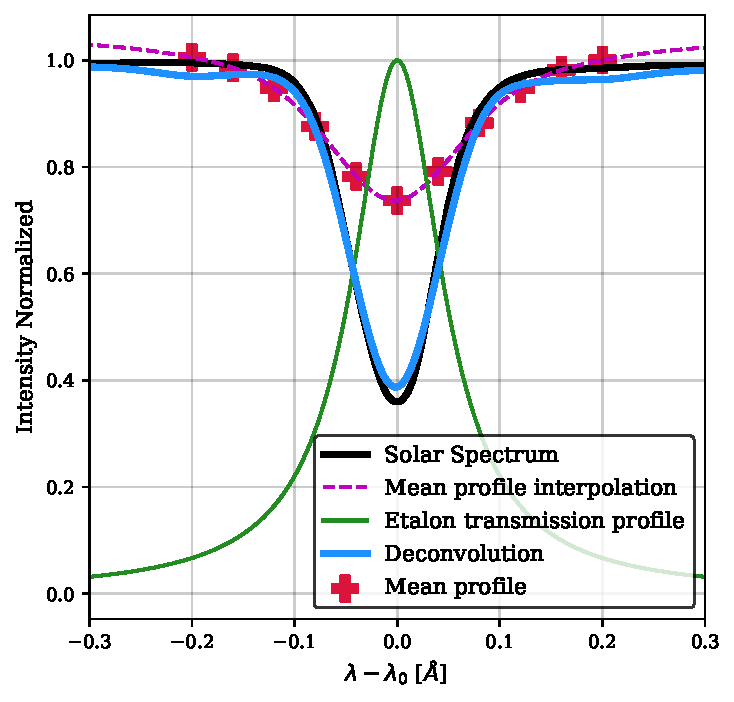
\includegraphics[width=\textwidth]{figures/EtalonPaper/Deconvolution.pdf}
\caption[Object deconvolution.]{Deconvolution of the object with a measurement of the Fe I spectral line using $N_\lambda = 9$. All points of the FoV have been used to compute the average profiles (blue crosses). The deconvolution (orange) is the result of deconvolving the mean profile interpolation (dashed line) with the displayed etalon transmission profile (red).\label{fig_etalon_corr:Deconvolution} }
\end{figure}

We employed Newton's method to minimize the merit function, Eq.~\eqref{eq_eta_corr: Merit Function}, as it has been proven to quickly converge (in five iterations or fewer, usually). The method begins by assuming an initial guess for the gain $g_j$ and $\Delta a_j$ parameters. Then, provided the initial guess is sufficiently close to the solution and that the merit function is continuous and differentiable, the gain $g_j$ and $\Delta a_j$ encoded in the vector, $\mathbf{x}_j$, can be updated iteratively at each iteration, $j$, as

\begin{equation}
\mathbf{x} _ {j + 1} = \mathbf{x} _ j - \mathcal{H} ^ {- 1} \mathcal{J} ^ T f(\mathbf{x}_j) \ , 
\end{equation}

where $\mathcal{H}$ and $\mathcal{J}$ are the Hessian and Jacobian matrices of the merit function $f$, respectively, calculated for $\mathbf{x}_j = [g_j,\Delta a_j]^T$, and $T$ stands for the transpose. Hence, the transmission profile of the etalon and its derivatives have to be computed for every wavelength and every pixel at each iteration. This can be computationally costly, especially when using imperfect telecentric configurations, where numerical integrals are involved. All derivatives needed for the algorithm are calculated analytically, except when simulating imperfect telecentrism. A detailed formulation of these derivatives is provided in the appendix.

Regarding the object $O(\lambda)$, if we assume it is given by the solar atlas, no additional computations are needed. However, when using the deconvolution approach, the object has to be calculated in each iteration. In this case, the algorithm works as follows: First, we compute the average profile across the whole FoV, and we force the continuum intensity to be the same on both sides of the spectral range to reduce the boundary effects of the deconvolution. This step is only necessary in case the spectral line is sampled in only a few positions, as is the case of the SO/PHI, IMaX, or TuMag instruments, where only a continuum point, either at the red or the blue side of the spectrum, is recorded. Both the object and transmission profile require a good spectral sampling to accurately compute the integrals of Eq.~\eqref{eq_eta_corr: Error metric}. Second, a cubic spline interpolation is applied to the generated average profile to artificially improve the spectral sampling, if necessary. Finally, the interpolated profile is then deconvolved by means of a Wiener filter with the etalon's transmission profile. The result of this deconvolution is the object, $O(\lambda)$, used in the minimization algorithm. The deconvolution of the object is done every time the etalon defects are updated in order to improve the resemblance of the deconvolved object to the real one. Figure \ref{fig_etalon_corr:Deconvolution} shows an example of this process in a simulated observation using nine scanned points and a collimated configuration. The deconvolution manages to reproduce the original signal, with only some minor differences in the line core and the beginning of the wings.

\subsection{\label{eta_corr_susec: results}Test scenarios and results}

The aim of the simulations carried out in this section was to characterize the role of the noise $\delta _ i ^ {\lambda_s}$, the spectral sampling, the selection of the object $O(\lambda)$, and the accuracy of the method for both the collimated and telecentric configurations. All simulations were run for different choices of the number of scanned wavelengths, ranging from $N_\lambda=5$ to $N_\lambda=21$. 

\subsubsection{Impact of the noise level}
We first assumed that the spectrum of the observed object is given by the solar atlas. This way, all errors in the derivation of the gain and etalon defects only come from the noise introduced into the measurement. We refer to this as the "ideal case." Since we were combining different measurements taken at different wavelengths, we considered a worst-case scenario and simulated three different S/N: 100, 150, and 200. 

We restricted imperfections in the telecentrism to arise only for one scenario, S/N~$=200$, since simulating imperfections requires a high computational effort due to the lack of a theoretical expression for both the transmission profile and its derivatives. We also assumed that the degree of telecentrism ($0.3 ^\circ $) is known in this case.

\begin{figure}
    \centering
     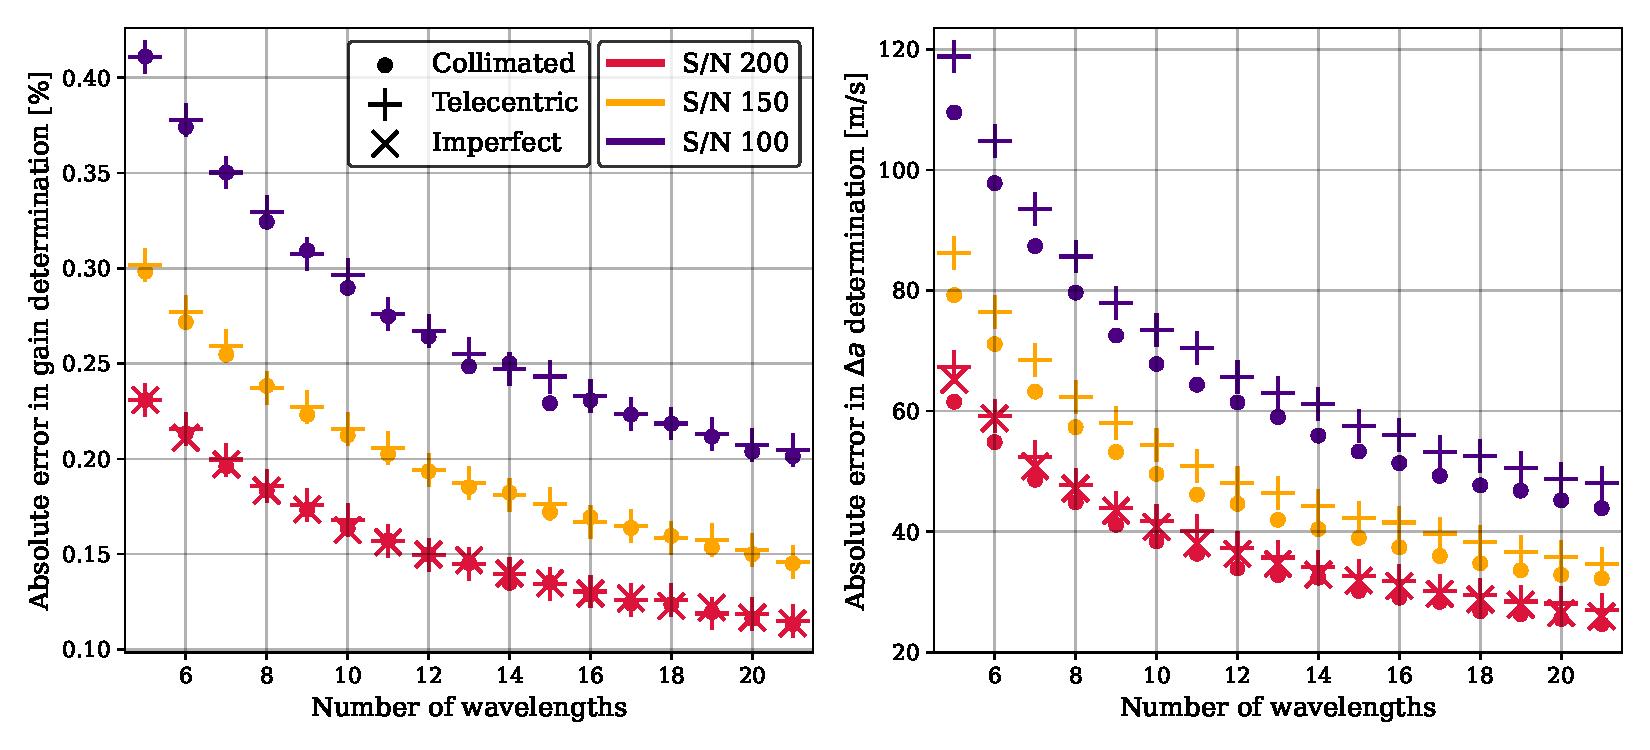
\includegraphics[width=\textwidth]{figures/EtalonPaper/SNR_plot_imperfect.pdf}
    \caption[Errors in etalon parameters derivation.]{Absolute errors of the gain (left) and etalon defect (right) derivations averaged over all the FoV. The number of wavelengths corresponds to the parameter $N_\lambda$ of wavelengths used to scan the profile.\label{fig_etalon_corr:SNR_both}}
\end{figure}

Figure \ref{fig_etalon_corr:SNR_both} shows the average absolute error in $g$ (left panel) and in $\Delta a$ (right panel) over the whole FoV as a function of the wavelength sampling, $N_\lambda$. The error in $g$ is expressed as a percentage of its real value. Errors in $\Delta a$ are given in meters per second since they are mostly responsible for shifting the profile. Errors in $\Delta a$ can be translated into velocity errors by computing the doppler velocity (Eq. \eqref{eq_spectro: Doppler}) associated to the spectral shift of the transmission peak produce by the error in $\Delta a$.

All the scenarios exhibit a similar behavior as far as their dependence on the spectral sampling is concerned, namely, the absolute errors decrease monotonically when the wavelength sampling increases. The reason for this is simply that a larger number of wavelength samples increases the amount of available information that the algorithm can use, thus making the fitting for $g$ and $\Delta a$ more precise. These results highlight the importance of properly sampling the targeted spectral line. A modest sampling of only $N_\lambda=5$ can produce errors as large as $120 \, {\rm ms^{-1}}$ in the worst-case scenario (S/N = 100). 

The noise level also plays an important role in the accuracy of the results. Scenarios with a lower S/N always have larger errors, for a given $N_\lambda$, in both the gain and $\Delta a $ computations. The difference in the performance of the algorithm due to the noise also changes with the spectral sampling; scenarios with a poor spectral sampling suffer from larger differences in the accuracy between the different S/N (50 ms$^{-1}$ for $N_\lambda$ = 5 between S/N = 200 and S/N = 100) than those with higher samplings (35 ms$^{-1}$ for $N_\lambda = 21$).

The optical configuration of the etalon has a very small impact on the accuracy of the algorithm. Results for the three setups are very similar, particularly in the gain calculation, for which the results are almost identical for all configurations. Retrieval of $\Delta a$ is slightly better for the collimated mount, though.

\begin{figure}
    \centering
    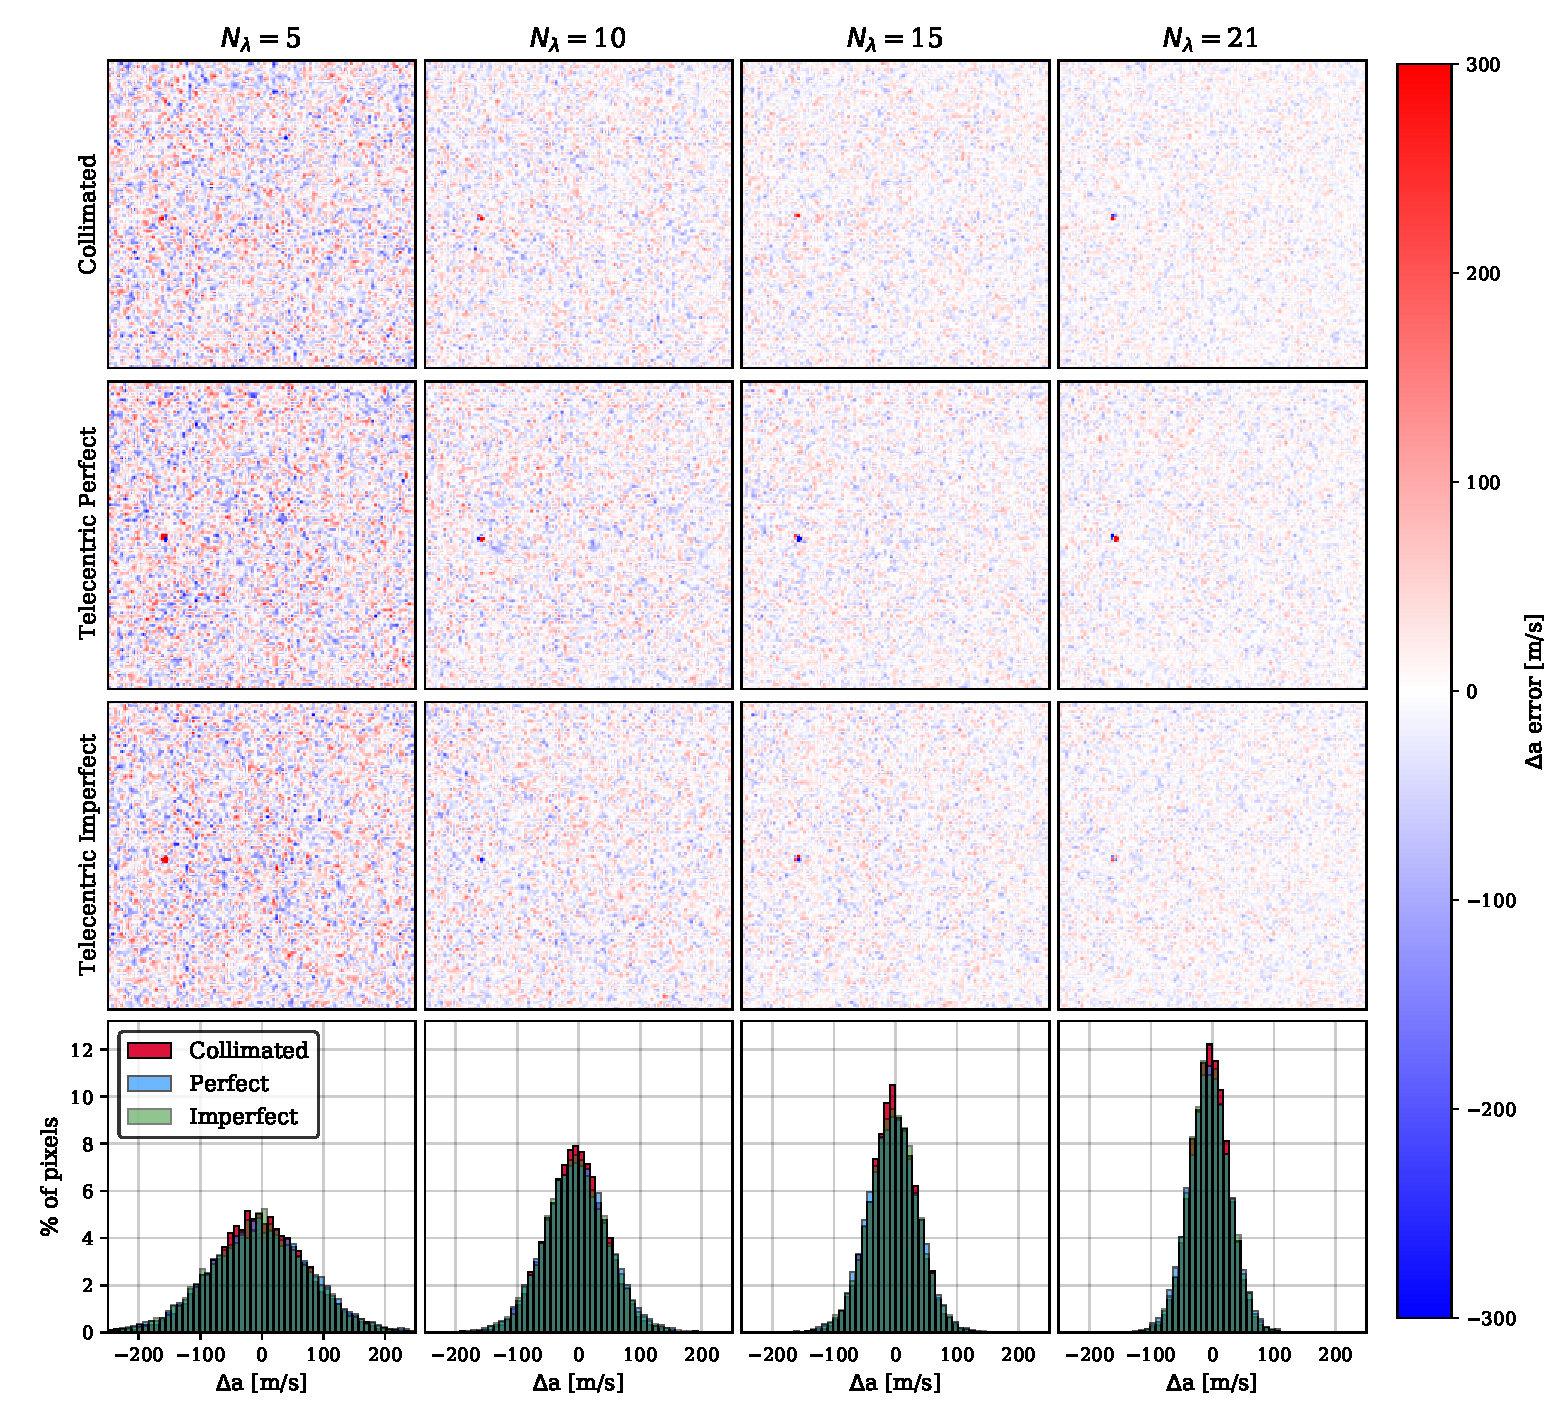
\includegraphics[width=\textwidth]{figures/EtalonPaper/Maps_Fov_Hist.pdf}
    \caption[Error distribution along the FoV,]{Distribution of the errors in the $\Delta a$ computation for the three configurations (first three rows) and different spectral samplings (columns). In the bottom panels of each column, the error distribution for the corresponding spectral sampling is shown for the three configurations. }
   \label{fig_etalon_corr:FOV}
\end{figure}

Figure \ref{fig_etalon_corr:FOV} shows the spatial distribution of the errors in the retrieval of $\Delta a$ for different choices of $N_\lambda$. There are no signs of a radial distribution in the maps shown in the figure, contrary to the actual distribution of the $\Delta a$ parameter, as shown in Fig.~\ref{fig_etalon_corr: Inputs}, right panel. This means that the precision of the method is similar no matter the amplitude of the defects, that is, we achieve the same accuracy in the retrieval of defects associated with shifts of 3 pm ($\sim$ 1450 ms$^{-1}$, near the corners of our FoV), which correspond to cavity errors of around 1.5 nm or incidence angles of approximately 0.4 degrees, and in the retrieval of regions where no defect is present (radius of 20 pixels from the center of the FoV approximately). Instead of a radial distribution, the errors follow a Gaussian-like distribution (shown at the bottom panels in \ref{fig_etalon_corr:FOV}) similar to the one followed by the noise contribution.

The standard deviation of the errors for both the gain and $\Delta a$ computations are also reduced with an increase in spectral sampling. The last row of Fig. \ref{fig_etalon_corr:FOV} displays the error distributions in the calculation of  $\Delta a$ for the three optical configurations and different spectral samplings. These results illustrate how the three configurations yield practically identical results and how the distribution narrows as $N_\lambda$ increases, thereby improving the results. Specifically, the standard deviation decreases from 50 ms$^{-1}$ for $N_\lambda = 5$ to 20 ms$^{-1}$ for $N_\lambda = 21$. In the case of the gain determination, the standard deviation ranges between 0.2 \% and 0.1\% for the scenarios with the poorest and highest spectral sampling, respectively.

\subsubsection{\label{sect: fitting_deconv}Impact of the object approximation}

To infer the error of the algorithm when the object is unknown, we compared the performance of the ideal case, that is, when the object used to generate the observations is known, with the one achieved when deconvolving the object from the data. Only the collimated setup was simulated in order to focus exclusively on the errors introduced by the deconvolution. The data has been degraded by Gaussian noise with an S/N = 200 in both scenarios. 

\begin{figure}
    \centering
     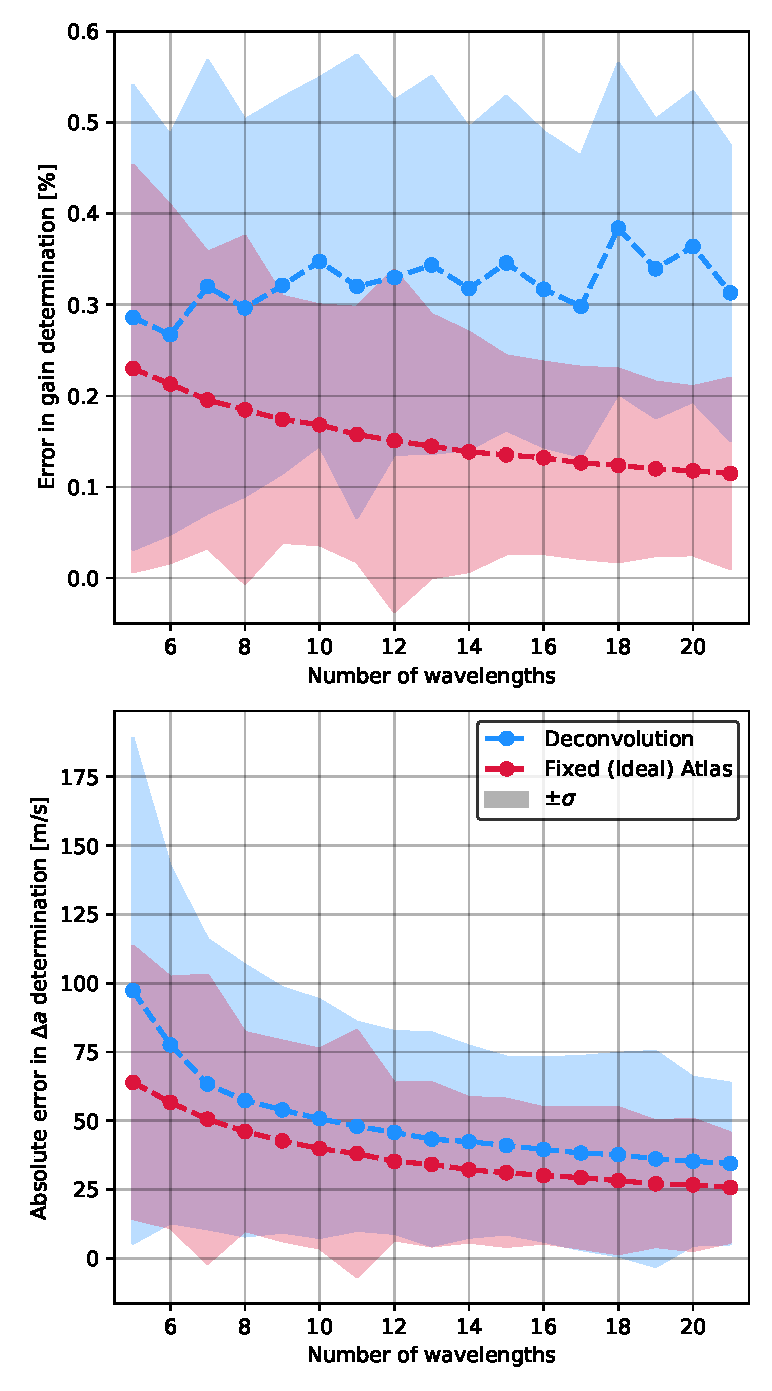
\includegraphics[width=\textwidth]{figures/EtalonPaper/Deconvolution_results.pdf}
    \caption[Errors for the deconvolution approach.]{Errors in gain determination and etalon properties averaged over all the FoV with a signal-to-noise ratio of 200 and a collimated configuration.}
    \label{fig_etalon_corr:Deconvolution-results}
\end{figure}

Figure \ref{fig_etalon_corr:Deconvolution-results} shows the results for the two approaches. Interestingly, the error in the gain for the deconvolution approach does not decrease with a larger number of wavelengths, unlike the ideal case. Nevertheless, the average error of the calculation is below 0.4~\%, with a dispersion (1 $\sigma$) of $\pm$ 0.3~\%. The deconvolution approach is prone to higher errors when deriving the gain due to the normalization of the profiles. The reason for this is two-fold. first, if the continuum is far enough from the spectral line, the normalization is strictly the integral over the transmission profile because the object is flat along the integration interval. However, this is not strictly true since the wings of the transmission profile can reach the spectral line (see Fig.~\ref{fig_etalon_corr: Prof-Measure}), hence modifying the normalization of the profile when the object changes at each iteration. Second, should the continuum intensity of the derived object vary with respect to its real value due to the deconvolution process (e.g., due to boundary effects), there will be a shift in the intensity of the whole profile induced by the normalization process. These two effects seem to dominate the accuracy on the gain determination, regardless of the chosen sampling.

For $\Delta a$, the performance of the method is slightly worse than for the ideal case when using the deconvolution approach. Unlike the gain determination, errors in the $\Delta a$ derivation show a strong dependence on the spectral sampling. Differences between both approaches range from $10$~ms$^{-1}$ to $40$~ms$^{-1}$ and increase with decreasing $N_\lambda$. The sensitivity with $N_\lambda$ is especially high up to $N_\lambda = 8$. A modest increase of $N_\lambda$ from five to six improves the determination of $\Delta a \sim$ 20 ms$^{-1}$, whereas at better spectral samplings, the difference between each simulation decreases more slowly, without any relevant improvement as the sampling increases. In any case, differences are all well within $\pm 1\sigma$.

\subsubsection{The crossover case}

The fact that the sensitivity of the model to the gain and to the $\Delta a$ parameters are different guarantees (to some extent) that the parameters can be separated from each other. The treatment of the problem is very different between etalon configurations, and therefore full knowledge of the setup is critical. However, this is not always feasible due to the unavoidable presence of errors, misalignment, and imperfections on the instrument. Approximations to describe the optical setup are also common in the pipeline of an FPI instrument because they reduce computational efforts. For instance, telecentric mounts are usually simplified as collimated setups, as the f-numbers employed in solar instruments are usually very large. Imperfections of telecentrism are commonly neglected, too. In this section, we analyze the impact of assuming an incorrect etalon mounting. To do so, we repeated the previous exercise, starting from a perfect and imperfect telecentric configuration but assuming that the transmission profile shape corresponds to a collimated one.    

\begin{figure}[t]
    \begin{minipage}[c]{0.6\textwidth}
      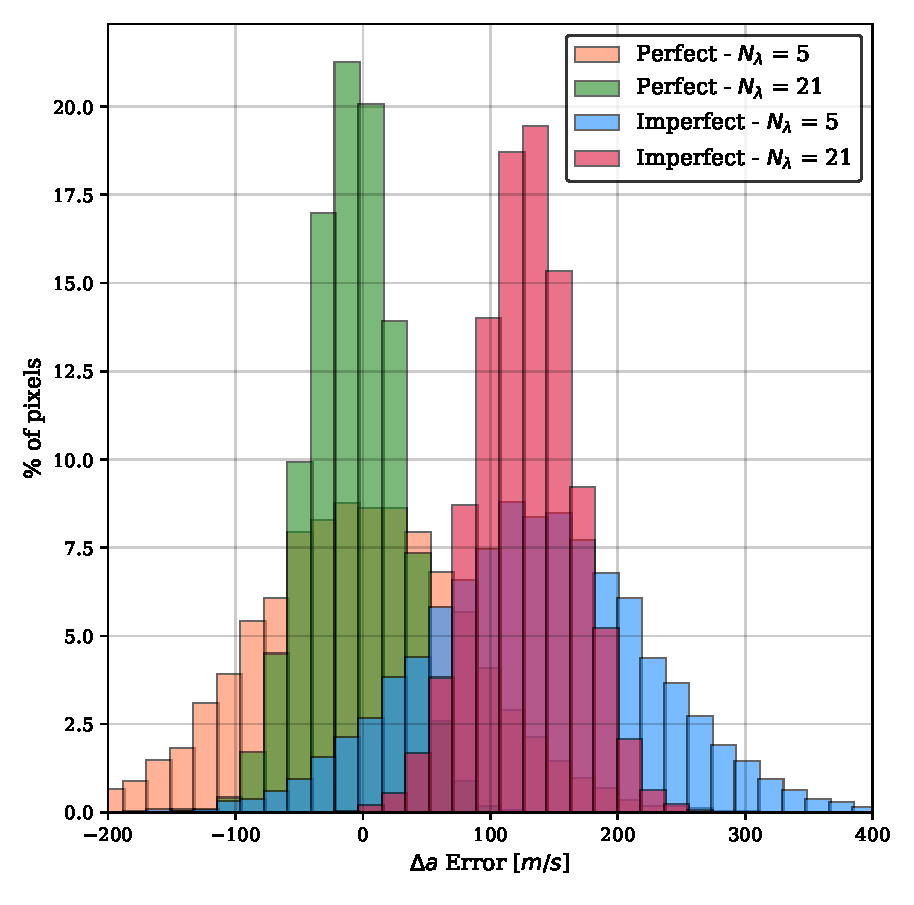
\includegraphics[width=\textwidth]{figures/EtalonPaper/histograms.pdf}
    \end{minipage}\hfill
    \begin{minipage}[c]{0.37\textwidth}
      \caption[Error distribution for imperfect telecentrism.]{
        Distribution of the errors in the determination of $\Delta a$ for the crossover scenarios (different configuration in the observation generation and minimization algorithm) for both perfect and imperfect configurations. Only results for the two extreme spectral samplings ($N_ \lambda = 5$ and $N_\lambda = 21$) are shown.
      } \label{fig_etalon_corr:Crossover_histograms}
    \end{minipage}
  \end{figure}

In this exercise, we assumed that we have an instrument with an FPI in a telecentric mount, as in the previous sections, in both perfect and imperfect configurations and an S/N~$=200$. We also considered that the object is given by the spectral solar atlas. The shift of the perfect telecentric transmission profile with respect to the collimated one was corrected using Eq.52 from \cite{franI} to avoid the emergence of spurious velocity signals. Imperfections in the telecentrism shift the profile more. This additional displacement was left uncorrected intentionally so we could study its effects.

Figure \ref{fig_etalon_corr:Crossover_histograms} shows the error distributions for $\Delta a$ when the model assumes a collimated configuration for $N_\lambda=5$ and $N_\lambda=21$ and for both perfect and imperfect configurations. The amplitude and dispersion of the error distributions are very similar for the two mounts and are comparable to the results obtained in the ideal case (Fig.~\ref{fig_etalon_corr:FOV}, bottom panel). The main difference between the perfect and imperfect scenarios is a shift of $130$ ms$^{-1}$ for the reason mentioned above. We note that this shift can easily be accounted for since it is a known and measurable effect. 

The similarity in the error distributions for the calculation of $\Delta a$ in the two scenarios demonstrates that the error incurred when assuming a collimated etalon does not significantly impact the determination of the cavity maps of the etalon. This is because changes in $\Delta a$ mostly induce a shift of the transmission peak by an equal amount in both cases.

\begin{figure}[t]
  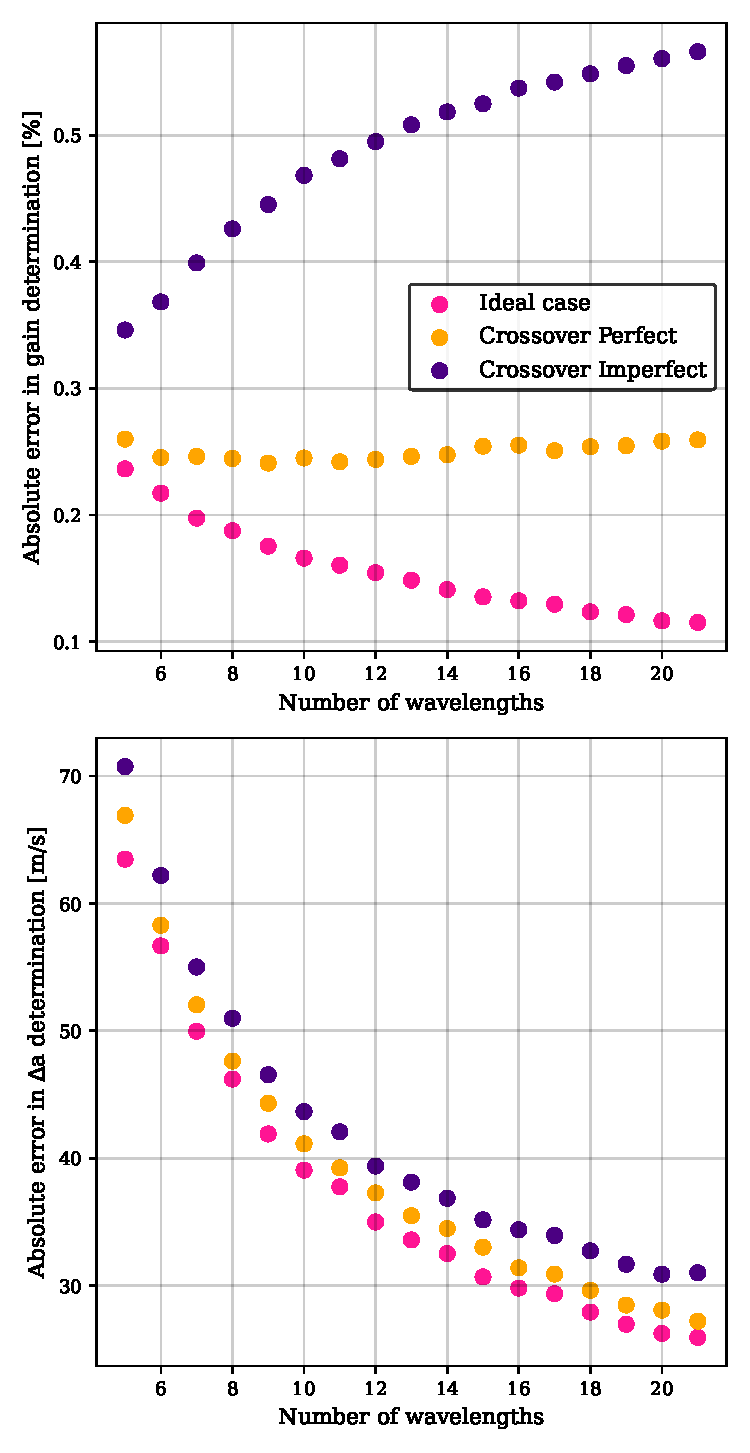
\includegraphics[width=\textwidth]{figures/EtalonPaper/means.pdf}
  \caption[Crossover case errors.]{Average errors of the gain (left) and etalon defect (right) calculations over all the FoV for the two crossover cases and the standard case (also shown in Fig.~ \ref{fig_etalon_corr:SNR_both} as the collimated case with S/N = 200) for reference. All $\Delta a$ errors have been computed by correcting differential offsets of the transmission profile between the different mounts.\label{fig_etalon_corr:crossover}}  
\end{figure}

We note, however, that the amplitude, width, and shape of the transmission profile differ significantly between the telecentric and collimated configurations, leading to an expected higher error in gain calculation. Figure \ref{fig_etalon_corr:crossover} shows the absolute errors in gain and $\Delta a$ calculations for both crossover scenarios and the ideal case after correcting the wavelength shift between the different mounts. For $\Delta a$, the performance of the method is very similar in the three setups, as also observed earlier. This behavior is nevertheless anticipated since the properties selected for simulating the imperfect etalon were chosen to mirror those of the SO-PHI etalon, which were adjusted to closely resemble the behavior of a collimated etalon to the greatest extent possible.

The differences are larger for the gain determination. Not only are the errors higher in the crossover cases, but the trend is entirely different. Instead of decreasing when increasing the number of wavelengths, gain errors remain the same for the perfect case and increase with the number of samples for the imperfect case. Similar to the deconvolution case (Fig.~\ref{fig_etalon_corr:Deconvolution-results}), the difference between transmission profiles introduces an error in the normalization process that systematically affects the rest of the measurements. This effect becomes more pronounced as the number of wavelengths increases, given that this error is introduced more frequently, and it is even more prominent in the imperfect case, as not only are the profiles different in this scenario, but they are also asymmetric. This asymmetry results in an imbalance in the measurement of the profile, as one wing of the spectral line has a higher transmissivity and is observed with greater intensity than the other.

Our results suggest that assuming an etalon in a collimated configuration for instruments with telecentric mounts can be a good first-order approximation for cavity map calculations, provided that the level of asymmetry of the transmission profile is known. However, achieving an accurate knowledge of the degree of telecentrism is often challenging in real instruments, as it usually varies across the FoV. Meanwhile, the results highlight that this approximation leads to a considerable increase in the error in the gain determination, which increases when increasing the spectral sampling. This contrasts with the standard philosophy of solar instrumentation, which requires a high number of points to better scan the spectral line.

\subsubsection{Real data}

While simulated tests are crucial for understanding the algorithm's behavior as a function of the different parameters of the problem, tests with real data are required to validate the effectiveness of the method. In this section, we evaluate the results obtained by the algorithm when implemented on observations acquired using the High-Resolution Telescope (HRT) of the SO/PHI instrument. 

The observation we used corresponds to a flat-field observation employing six points to scan the 6173 \r{A} line (five along the spectral line and an additional continuum measurement) conducted on March 9, 2022. The FPI aboard SO/PHI is illuminated in a telecentric mount, with an expected degree of telecentrism of about $0.3^\circ$. The tests conducted with this dataset have the same procedure as the ones employed for simulated data, that is, we only fit the gain and $\Delta a$ parameters, and we employed the deconvolution approach (Sect. \ref{sect: fitting_deconv}).

\begin{figure}[t]
  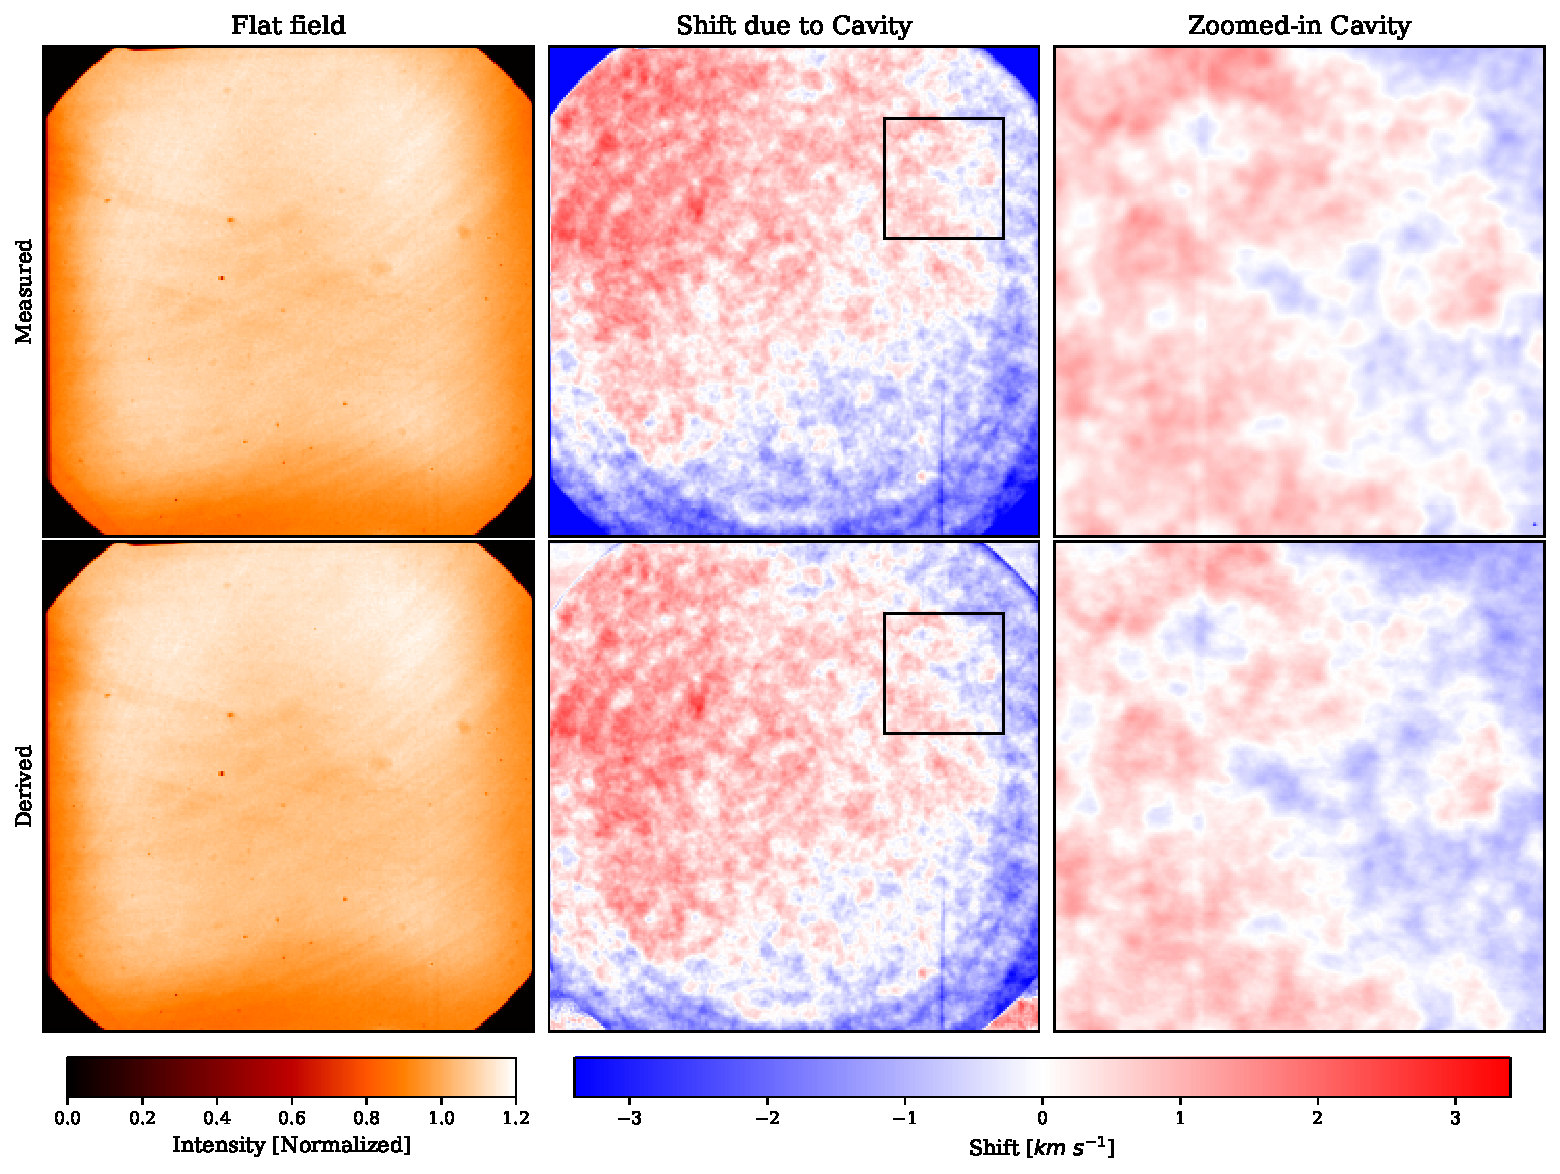
\includegraphics[width=\textwidth]{figures/EtalonPaper/Comparison_HRT.pdf}
  \caption[Comparison of results and real data.]{Comparison between the observed flat-field and cavity map (top row, left and center columns, respectively) and the derived flat-field (gain) and cavity map ($\Delta a$; bottom row, left and center columns, respectively). The right column in both rows showcases a zoomed-in region of each cavity map. The area corresponding to the zoomed-in region is indicated with a black square in the full cavity map to its left. The properties used to simulate SO/PHI's etalon are $R = 0.925$, $n=2.29$, $d = 251.63\ \mu m$, $f\# = 60$, $\Theta = 0.23 ^{\circ}$.\label{fig_etalon_corr:HRT}}  
\end{figure}

Figure \ref{fig_etalon_corr:HRT} shows the results obtained when applying the algorithm to HRT-SO/PHI data. The top row shows, from left to right, the observed flat at the continuum, the cavity map measured under laboratory conditions (on ground), and a selected region of the cavity map. In the bottom row, the same cases are shown but for the results inferred by the algorithm. That is, the flat-field (i.e., the gain) and the cavity map (i.e., $\Delta a$).

The results obtained for the cavity map closely resemble the laboratory measurements. The overall structure is preserved, maintaining the gradient from the upper left to the lower right. Similar structures are also discernible, such as the vertical line in the lower-right corner and the ring-like patterns evident in the lower section of the image. However, closer scrutiny of the observed structures revealed some differences. This deviation between results and measurements is expected, considering that the experiment conducted here represents a first-order approximation to assess the algorithm's capability to generate coherent results. Several factors contribute to these differences. Firstly, the spatial resolution of the cavity measured on ground is lower. Secondly, the degree of telecentrism has a predicted variation of $0.23^\circ$ across the FoV. Thirdly, we expected an error for the six-point scan, employing the deconvolution strategy, as large as a hundred meters per second.

Concerning the results for the gain determination, the comparison depicted in Fig.~ \ref{fig_etalon_corr:HRT} suggests that pixel-to-pixel gain variations can also be determined accurately with our method, as both small-scale and large-scale variations are reproduced with detail. 

\begin{figure}[t]
  \centering
  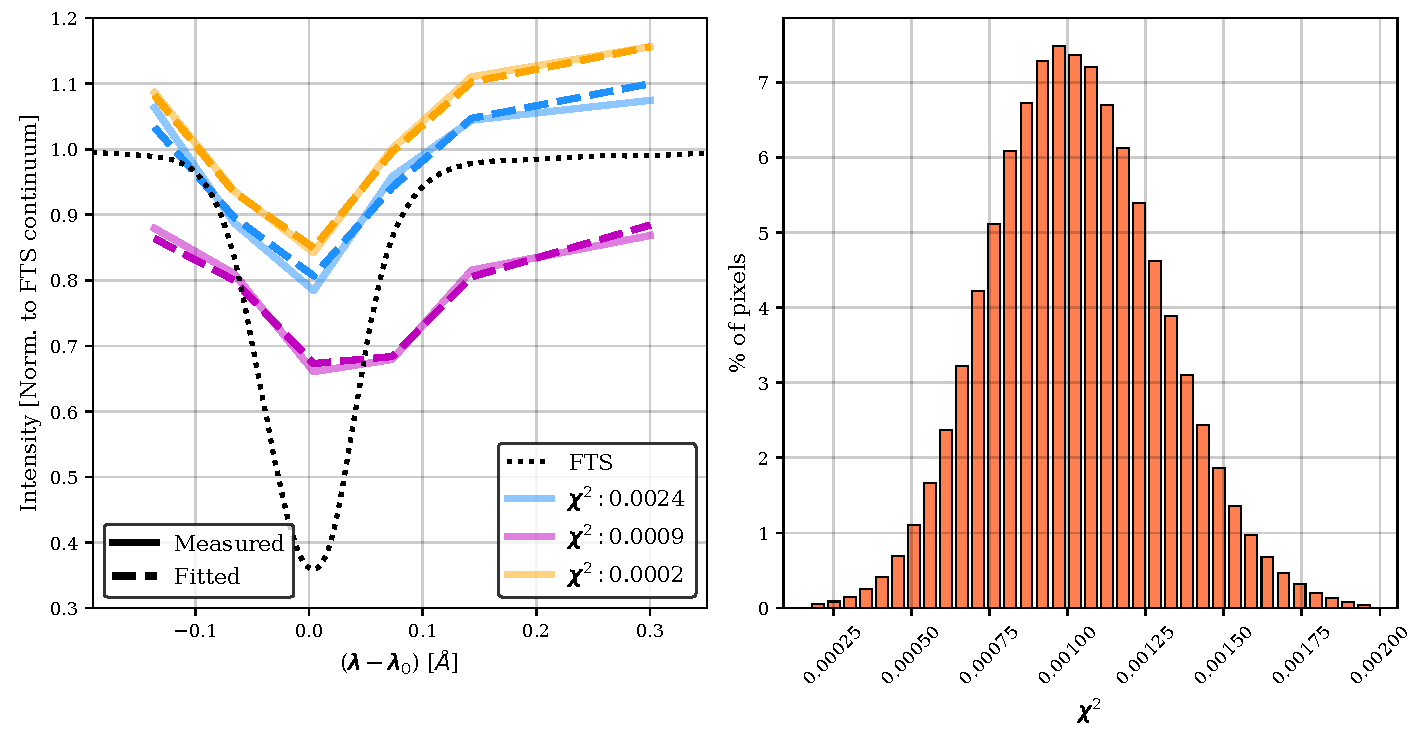
\includegraphics[width=\textwidth]{figures/EtalonPaper/fitting_chisq_hor.pdf}
  \caption[Fitting accuracy.]{Comparison between the measured (solid lines) and fitted profiles (dashed lines) for three pixels, each representing varying degrees of accuracy (left panel). The FTS is shown as a reference. The right panel displays the distribution of $\chi^2$ values for all pixels. Among the three selected cases, one demonstrates an average fit (depicted in pink, with $\chi^2$ close to the mean value), while the other two correspond with extreme cases—one with a notably good fit and the other with a poor fit (depicted in yellow and blue, respectively). The value for $\chi ^2$ has been computed employing equation \eqref{eq_eta_corr: Merit Function}\label{fig_etalon_corr: xisq_hrt}}  
\end{figure}

A more quantitative analysis of the results is depicted in Fig.~\ref{fig_etalon_corr: xisq_hrt}. The left panel shows a comparison between the fitted and observed profiles for three distinct cases with varying degrees of precision, while the right panel shows the distribution of $\chi^2$ for all pixels. In the worst-case scenario, small differences between the real profile and the fit can be seen in both the line wing and the line core. In any other case, the fittings are rather satisfactory.






